\chapter{Soluzione proposta}
\label{SoluzioneProposta}
\thispagestyle{empty}

\vspace{0.5cm}

\noindent In questo capitolo descriviamo la soluzione che abbiamo proposto per risolvere il problema del tampering detection, formulato nel Capitolo \ref{FormulazioneProblema}.\\
Nel Paragrafo \ref{indicatori} descriviamo quali sono gli indicatori che abbiamo deciso di monitorare per individuare gli eventi di tampering.\\
Nel Paragrafo  \ref{monitoraggio} illustriamo in che modo vengono monitorati questi indicatori in modo da individuare degli eventi specifici.\\
Nel Paragrafo \ref{segmentazione} descriviamo, infine, l'algoritmo di segmentazione che utilizziamo, assieme al monitoraggio, per individuare eventi di spostamento della camera.
\section{Indicatori utilizzati per identificare gli eventi di tampering}
\label{indicatori}
L'approccio che abbiamo considerato per risolvere il problema del tampering detection consiste nell'estrarre, da ciascun frame ripreso dalla camera, degli indicatori \textit{scalari} che possano essere monitorati nel tempo, in modo da individuare un cambiamento nel loro comportamento associabile a un evento di tampering. 
In particolare abbiamo deciso di considerare un indicatore in grado di verificare la presenza di sfocature globali all'interno della scena e un altro in grado di identificare gli eventi di spostamento della camera.
Il resto del paragrafo \`e dedicato alla descrizione di questi indicatori.
\subsection{Misura della sfocatura nell'immagine}
Nel Paragrafo \ref{sfocatura} abbiamo modellizzato il fenomeno della sfocatura secondo la formula \eqref{blur_multi}:
\[z_t(x)=\mathcal{D}_t[y_t](x) = \mathcal{B}_t[y_t](x) + \eta(x), \qquad x \in \mathcal{X}.\]
Ricavare un indicatore in grado di misurare direttamente il grado di sfocatura di un'immagine \`e difficile.
Quello che \`e possibile fare, come proposto in \cite{alippi2010detecting}, \`e utilizzare una misura \textit{indiretta} di questo operatore.\\
Come abbiamo visto nel Paragrafo \ref{sfocatura}, l'operatore di sfocatura $\mathcal{B}$ ha come effetto principale quello di rendere le differenze di intensit\`a tra pixel adiacenti pi\`u morbide (\textit{smooth}).
In base a questo \`e possibile identificare un evento di sfocatura andando a monitorare l'\textit{energia media del gradiente} di ciascuna immagine:
\begin{equation}
\label{eq:energyGradient}
g_t = \mathcal{G}[z_t] =\frac{\sum_{\mathcal{X}}\| \nabla z_t(x) \| _2^2 }{|\mathcal{X}|} ,
\end{equation}  
dove abbiamo indicato con $|\mathcal{X}|$ la \textit{cardinalit\`a} dell'insieme dei pixel $\mathcal{X}$, e con $\|\cdot\|_2$ la norma di tipo $\mathcal{L}_2$\footnote{$\|x\|_2=\sqrt{\sum_{t}x_t^2}$}.\\
Lavorando nel dominio discreto delle immagini digitali, possiamo calcolare le derivate dell'intensit\`a luminosa (\textit{luma}) per mezzo di convoluzioni con filtri derivativi.
In particolare, per il calcolo delle derivate orizzontali  abbiamo utilizzato il seguente filtro $f_i$:
\[f_i = f \circledast \left[ \begin{array}{rcl}
1 & 0 & -1
\end{array}\right], \] 
mentre per il calcolo delle derivate verticali  abbiamo utilizzato il seguente filtro $f_j$:
\[f_j = f \circledast \left[ \begin{array}{r}
1 \\ 0 \\ -1
\end{array}\right], \]
dove abbiamo indicato con $\circledast$ l'operatore di convoluzione e con $f$ un \textit{filtro gaussiano} di dimensione $5 \times 5$:
\[f(i,j)=\frac{1}{2\pi\sigma^2}\exp\left(-\frac{\left(i-k-1\right)^2+\left(j-k-1\right)^2}{2\sigma^2}\right)\] 
dove $k=2$ e  la deviazione standard $\sigma = 1$.
Con questi filtri \`e possibile calcolare la \textit{norma del gradiente} nel seguente modo:
\[\| \nabla z_t(x) \|_2^2=\left(z_t \circledast f_i\right)(x)^2 + \left(z_t \circledast f_j\right)(x)^2.\]
Una volta calcolata la norma del gradiente \`e possibile farne la media come specificato nella formula \eqref{eq:energyGradient}.
Il risultato finale \`e un indicatore \textit{scalare} per ciascun frame acquisito, che pu\`o essere monitorato per individuare eventi di sfocature. 
In particolare l'evento \`e associato a un \textit{crollo} del valore di $g$.
\subsection{Misura dello spostamento della camera}
Nel Paragrafo \ref{displacement} abbiamo modellizzato il fenomeno dello spostamento della camera secondo la formula \eqref{eq:displacement}
\[z_t(x)  = \left\{ \begin{array}{rcl}
y_t(x) + \eta(x) & \mbox{per} & t < T^* \\
w_t(x) + \eta(x) & \mbox{per} & t \geqslant T^*
\end{array}\right. , x \in \mathcal{X}\]
dove $T^*$ indica l'istante in cui avviene il cambiamento.\\
Uno spostamento della camera, quindi, \`e associato a un cambiamento \textit{globale} dei valori di intensit\`a luminosa (\textit{luma}) nei pixel dell'immagine.
In base a questo \`e possibile identificare un evento di spostamento della camera andando a monitorare l'\textit{energia media della luma} di ciascuna immagine:
\begin{equation}
\label{eq:energyLuma}
l_t = \mathcal{L}[z_t] =\frac{\sum_{\mathcal{X}} z_t(x) }{|\mathcal{X}|} ,
\end{equation}  
dove abbiamo indicato con $|\mathcal{X}|$ la \textit{cardinalit\`a} dell'insieme dei pixel $\mathcal{X}$.\\
Il risultato finale \`e un indicatore \textit{scalare} per ciascun frame acquisito, che pu\`o essere monitorato per individuare eventi di spostamenti della camera. 
\subsection{Comportamento degli indicatori nel tempo}
\label{comportamento}
\begin{figure}[tb]
	\centering
	\begin{subfigure}[]
		{\label{fig:FTgiorno} 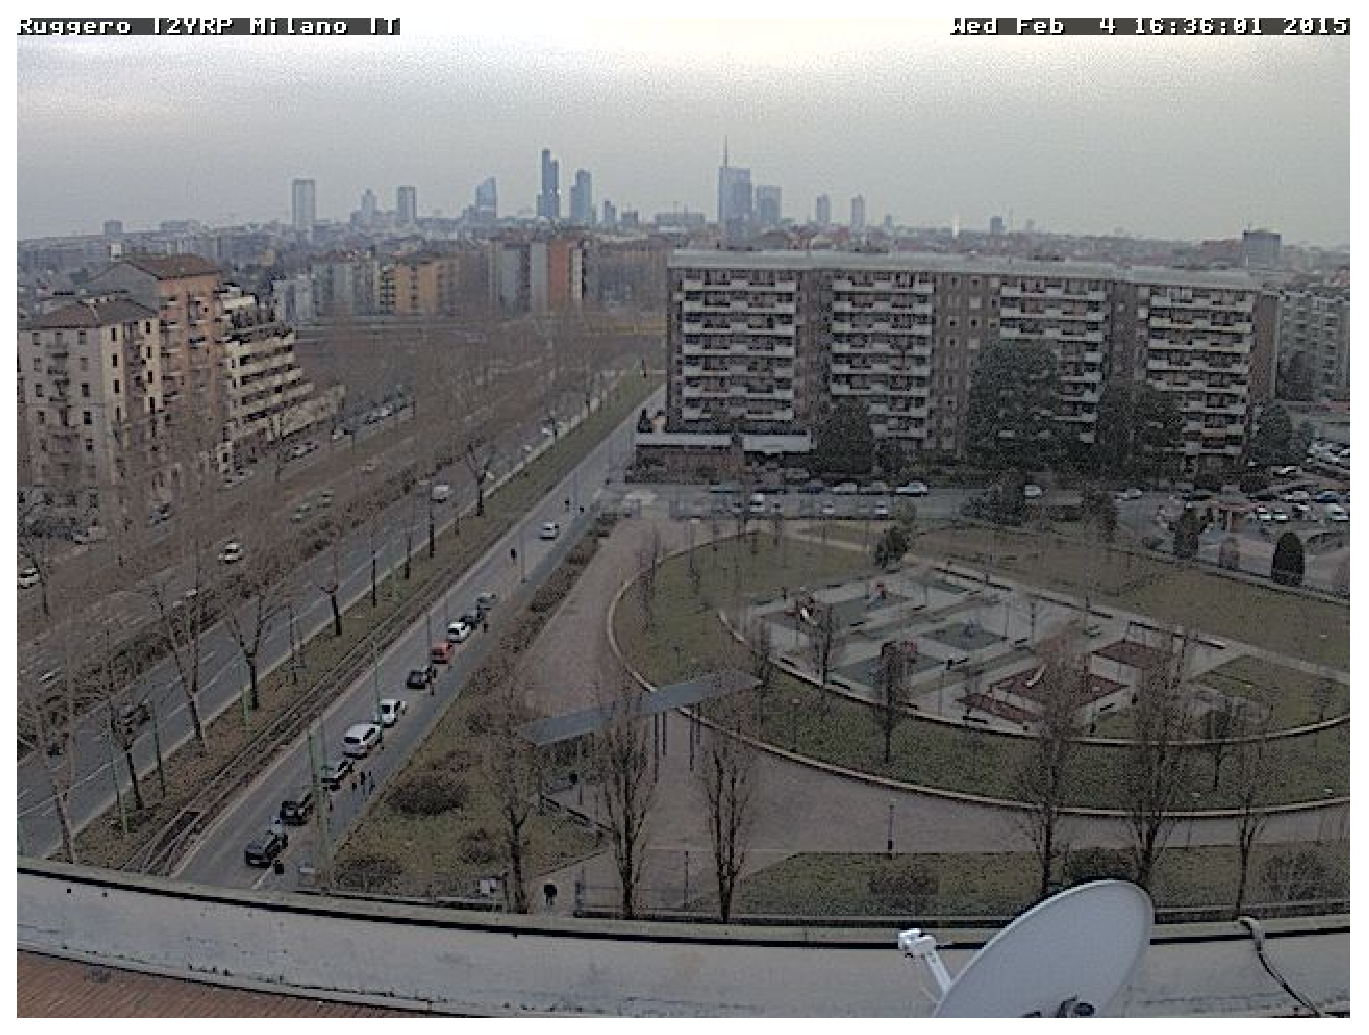
\includegraphics[width=6cm]{./pictures/testiGIORNO}}
	\end{subfigure}
	\begin{subfigure}[]
		{\label{fig:FTnotte} 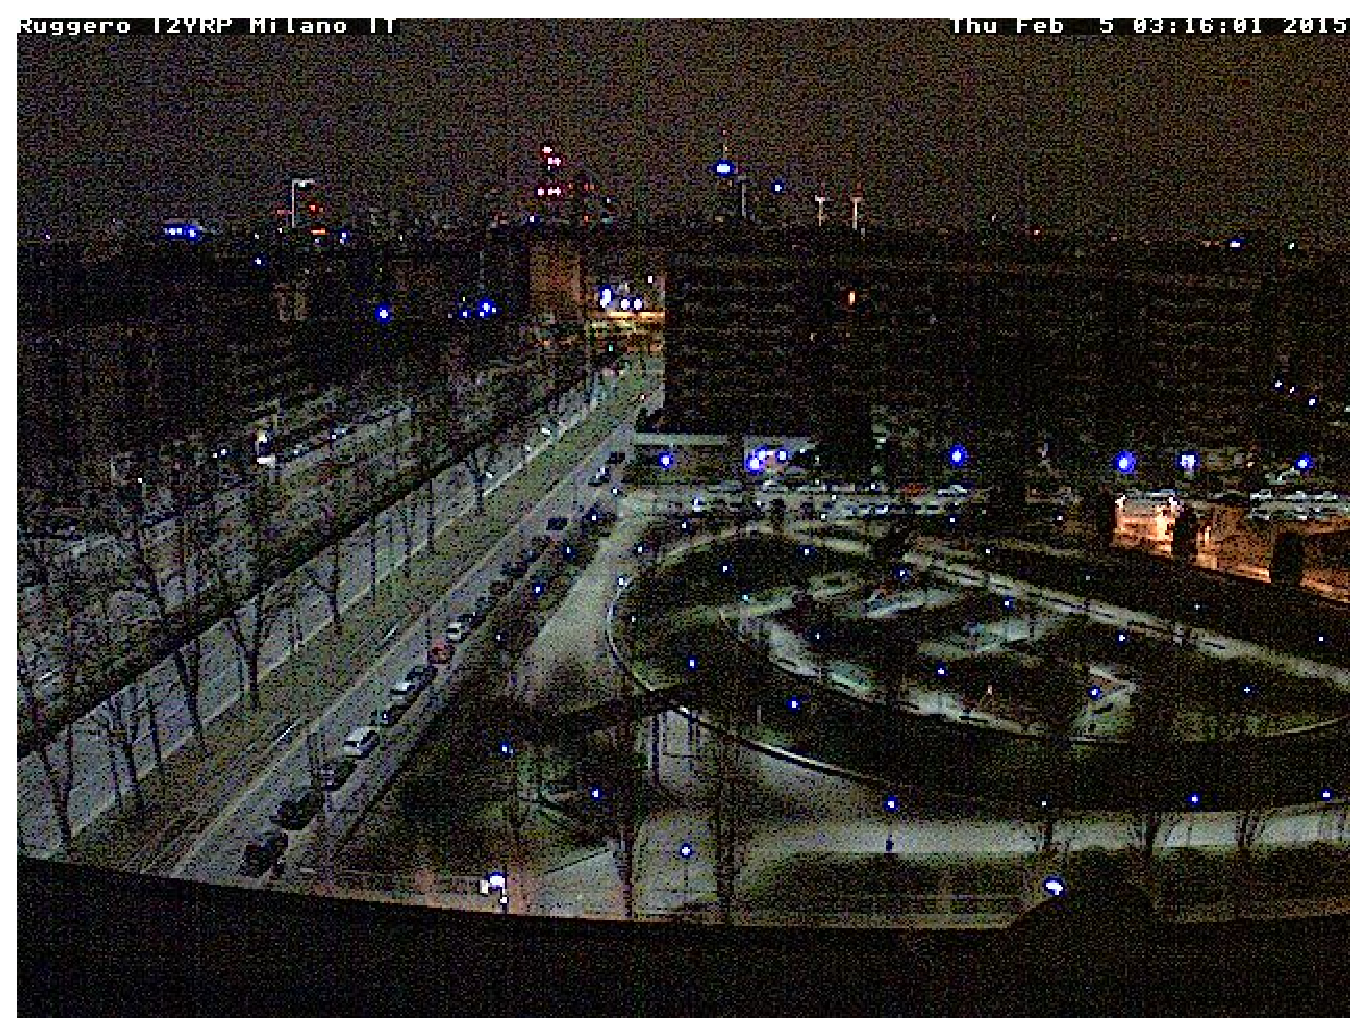
\includegraphics[width=6cm]{./pictures/testiNOTTE}}
	\end{subfigure}
	\caption{Esempio di cambi di luminosit\`a tra il giorno e la notte}
	\label{fig:testiGN}
\end{figure}
\begin{figure}[tb]
	\centering
	\begin{subfigure}[]
		{\label{fig:BAgiorno} 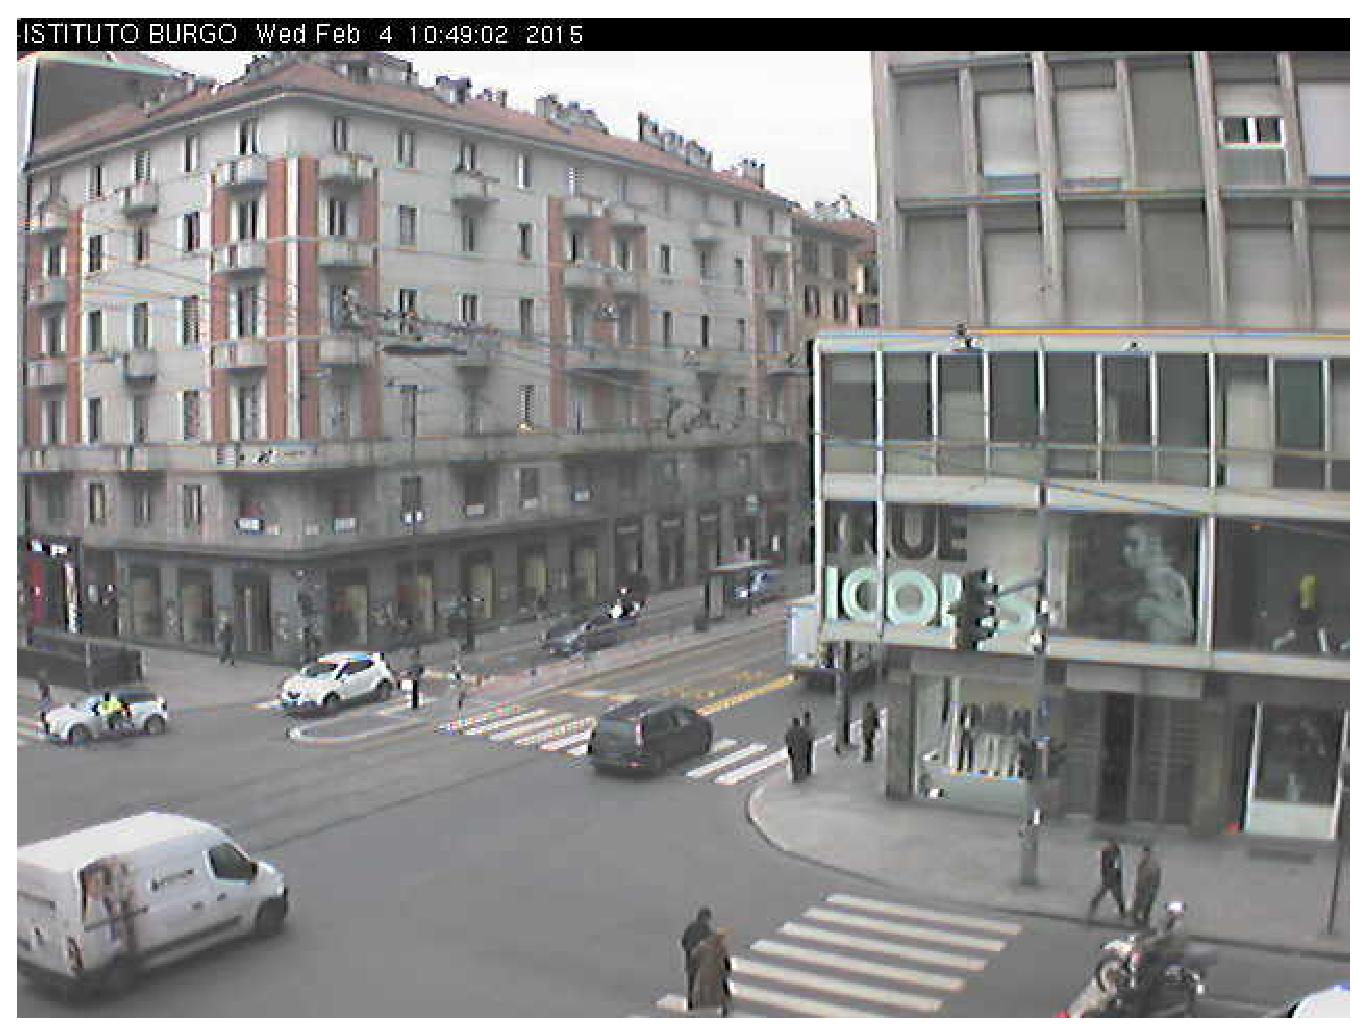
\includegraphics[width=6cm]{./pictures/buenosAiresGIORNO}}
	\end{subfigure}
	\begin{subfigure}[]
		{\label{fig:BAnotte} 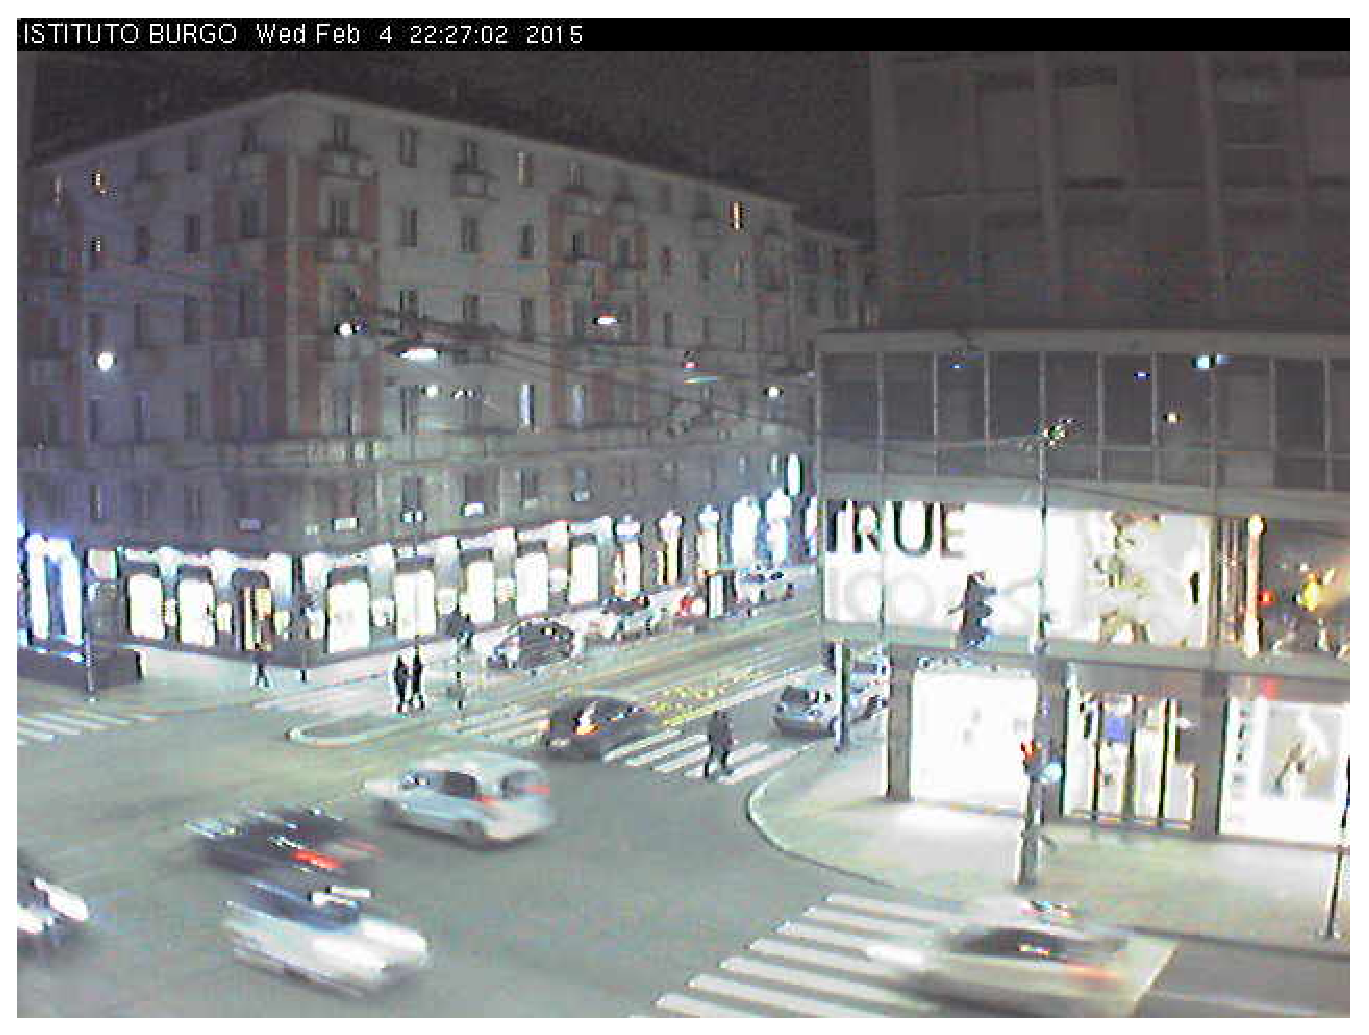
\includegraphics[width=6cm]{./pictures/buenosAiresNOTTE}}
	\end{subfigure}
	\caption{Esempio di presenza di sfocature dovute all'aumento del tempo di esposizione della camera}
	\label{fig:buenosAiresGN}
\end{figure}
Analizzando alcune sequenze video abbiamo notato che, anche in assenza di eventi di tampering, vi sono alcuni fattori che sono in grado di far variare il valore degli indicatori estratti.
Tra i pi\`u importanti abbiamo:
\begin{itemize}
	\item \textit{Cambi di luminosit\`a} che avvengono nel corso della giornata. 
	Se consideriamo l'esempio in Figura \ref{fig:testiGN}, possiamo notare come, nel passaggio dal giorno (Figura \ref{fig:FTgiorno}) alla notte (Figura \ref{fig:FTnotte}), le differenze di luminosit\`a siano elevate.  
	\item \textit{Dinamicit\`a della scena}. La ripresa di una scena movimentata, come ad esempio una strada, ha come risultato che ciascun frame sia diverso dagli altri.
	Ci\`o si traduce in una variabilit\`a elevata degli indicatori che abbiamo utilizzato. 
	Inoltre, col passare del tempo, pu\`o succedere che cambi anche il \textit{grado di dinamicit\`a} della scena.
	Considerando ancora l'esempio della strada, infatti, avremo dei momenti in cui il traffico \`e pi\`u intenso (nelle cosiddette \textit{ore di punta}) e altri in cui le macchine passano meno spesso (tipicamente durante la notte).
	\item \textit{Configurazione automatica della camera}. Solitamente le camere sono in grado di configurare in maniera automatica alcuni parametri, in base alle condizioni di luminosit\`a esterne.
	Ad esempio, durante la ripresa di scene notturne la camera solitamente aumenta il \textit{tempo di esposizione} del sensore, in modo da ricevere pi\`u luce possibile.
	Ci\`o si traduce in un \textit{aumento del rumore} su tutta la scena acquisita (come vediamo nel frame in Figura \ref{fig:FTnotte}) e in una \textit{presenza di sfocature} quando vengono immortalati degli oggetti in movimento (come ad esempio le macchine che si muovono nella Figura \ref{fig:BAnotte}).
\end{itemize} 
\begin{figure}[tb]
	\centering
	\begin{subfigure}[]
		{\label{fig:energy} 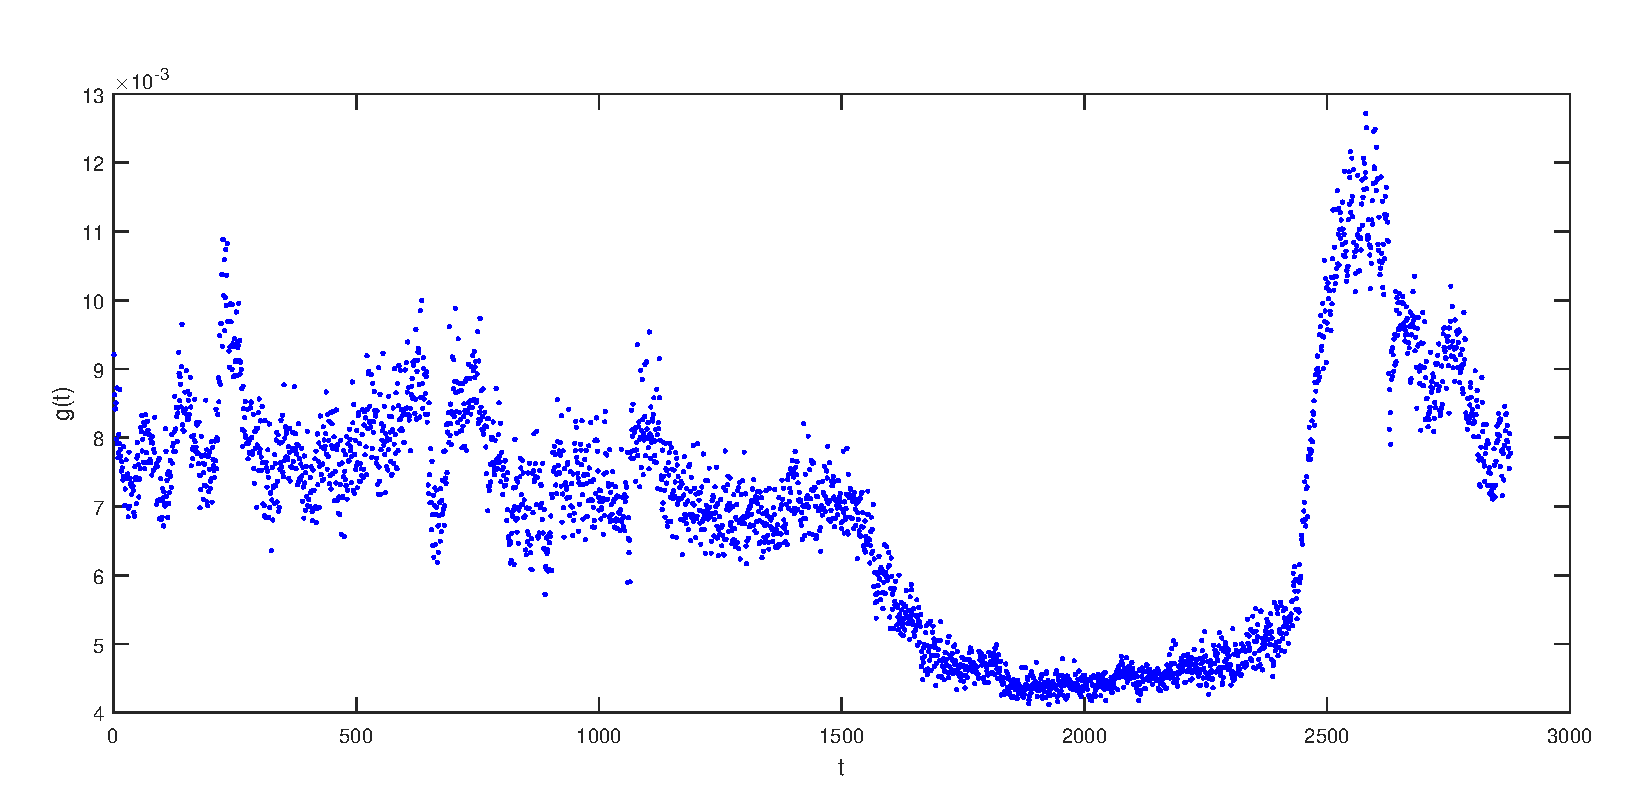
\includegraphics[width=12cm]{./pictures/energyTot}}
	\end{subfigure}
	\begin{subfigure}[]
		{\label{fig:energyDetr} 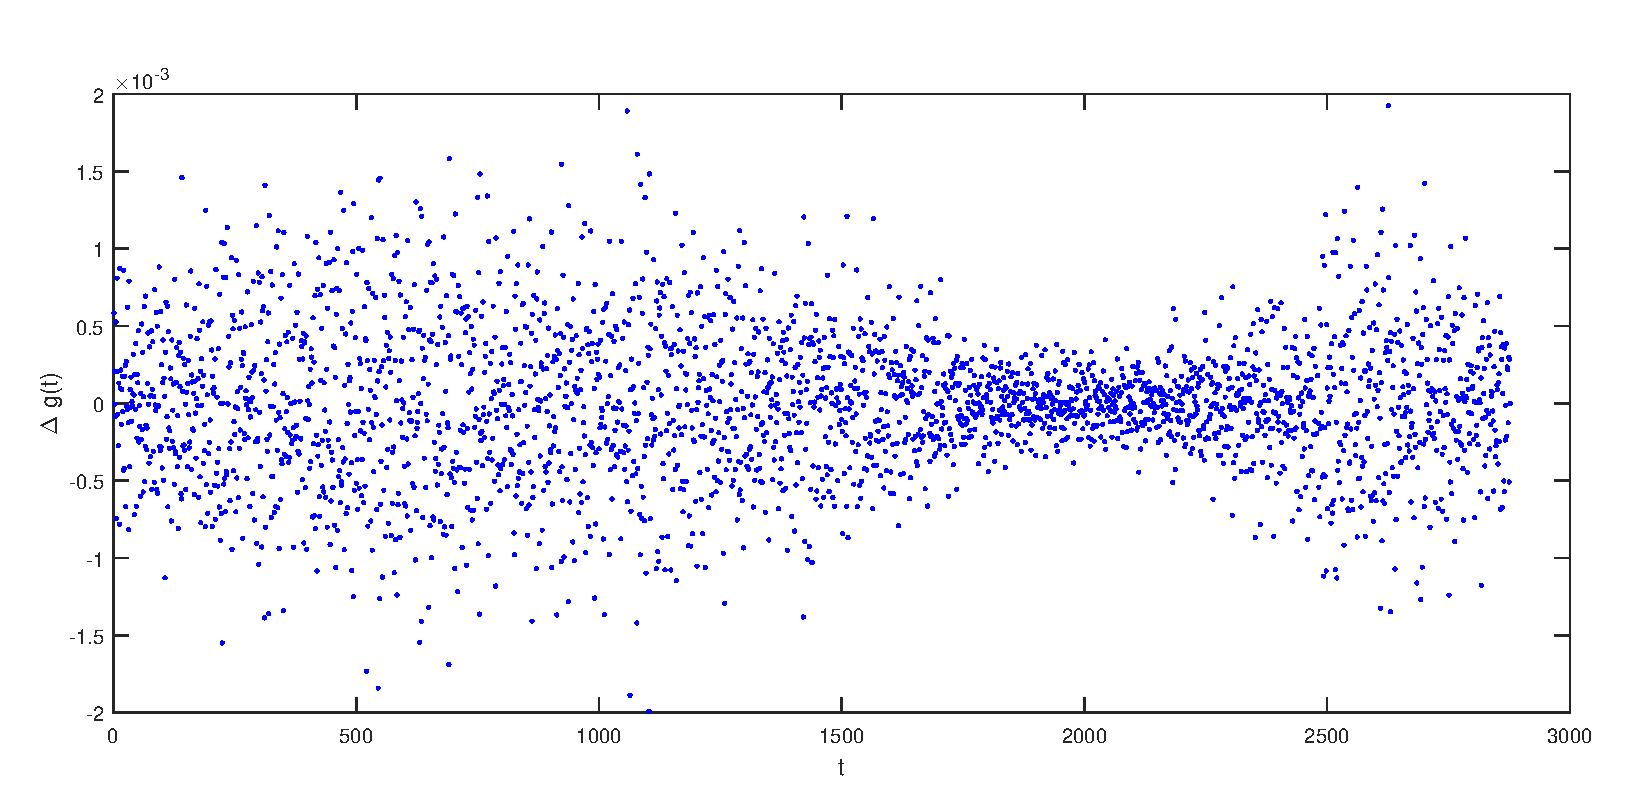
\includegraphics[width=12cm]{./pictures/energydetr}}
	\end{subfigure}
	\caption{Energia media del gradiente lungo un'acquisizione di 24 ore (a) e suo detrending (b)}
	\label{fig:energyTot}
\end{figure}
\begin{figure}[tb]
	\centering
	\begin{subfigure}[]
		{\label{fig:luma} 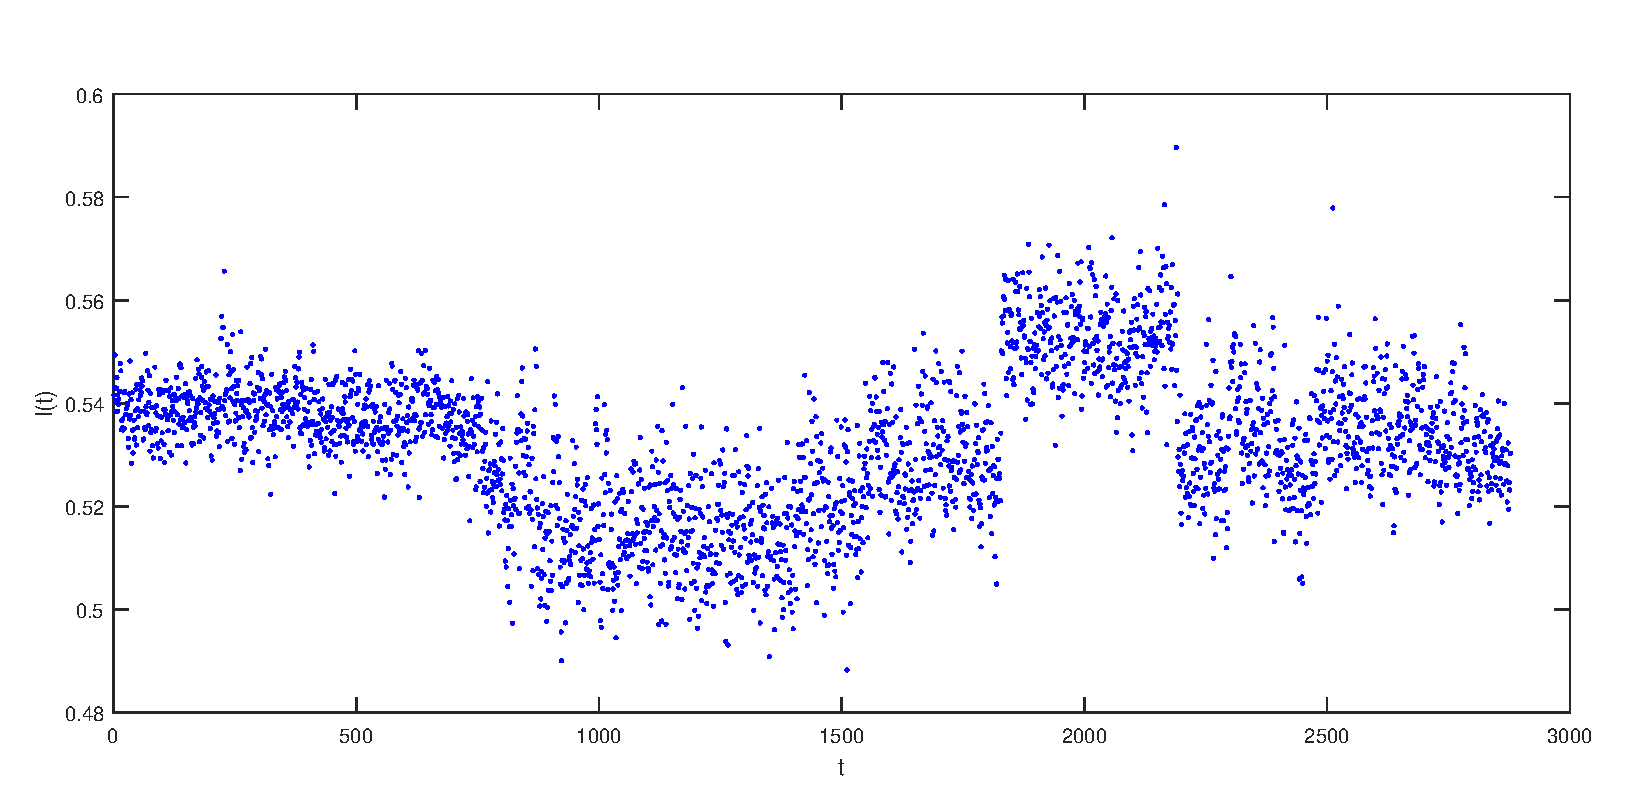
\includegraphics[width=12cm]{./pictures/lumaTot}}
	\end{subfigure}
	\begin{subfigure}[]
		{\label{fig:lumaDetr} 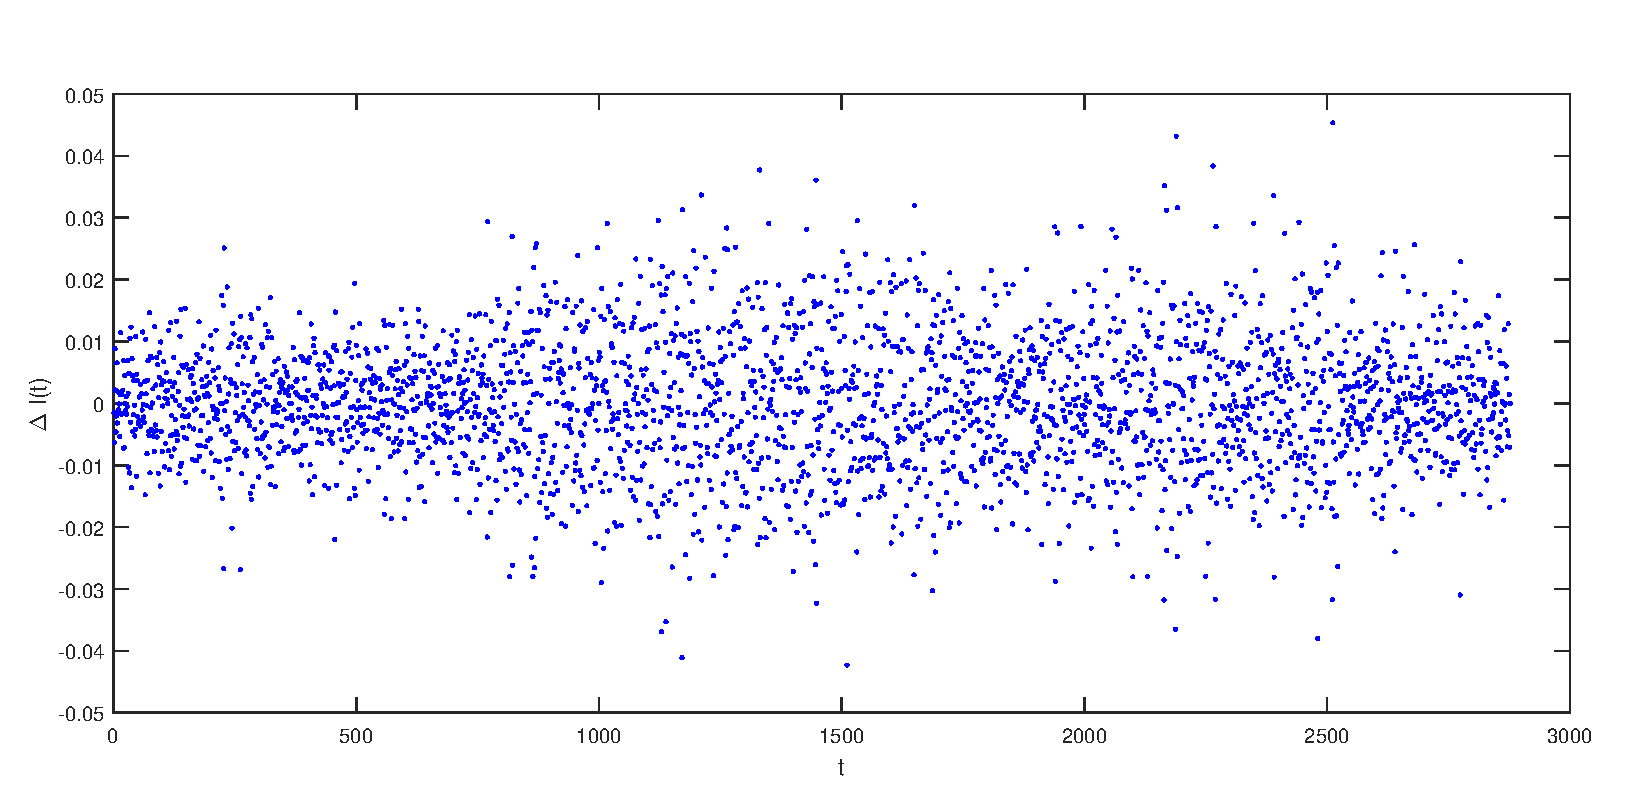
\includegraphics[width=12cm]{./pictures/lumadetr}}
	\end{subfigure}
	\caption{Energia media della luma lungo un'acquisizione di 24 ore (a) e suo detrending (b)}
	\label{fig:lumaTot}
\end{figure}
\begin{figure}[tb]
	\centering
	\begin{subfigure}[]
		{\label{fig:energyDefocus} 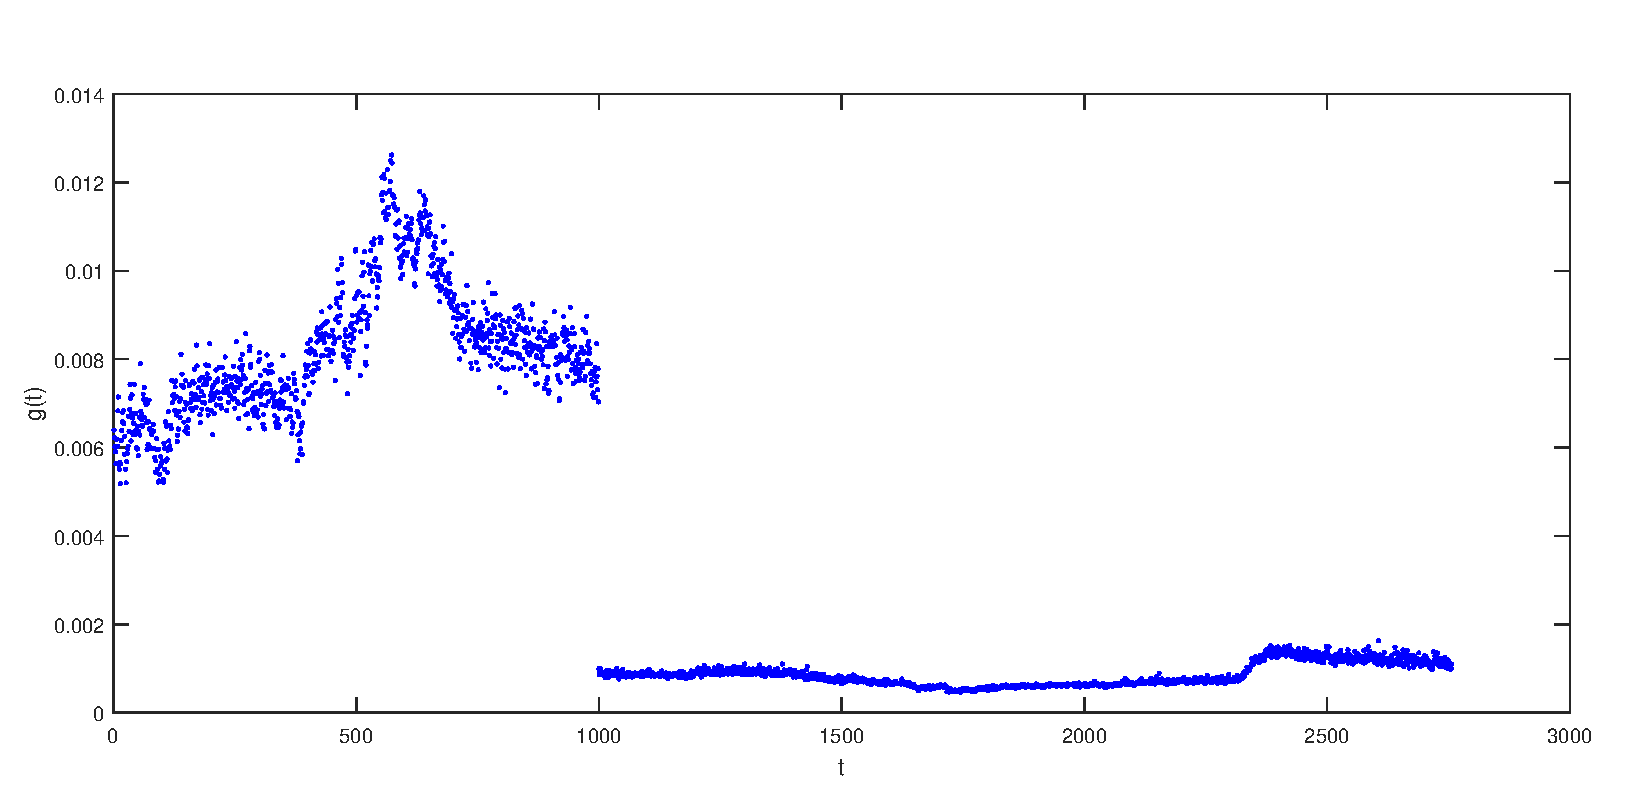
\includegraphics[width=12cm]{./pictures/Defocus/DEFOCUS_energy}}
	\end{subfigure}
	\begin{subfigure}[]
		{\label{fig:energyDetrDefocus} 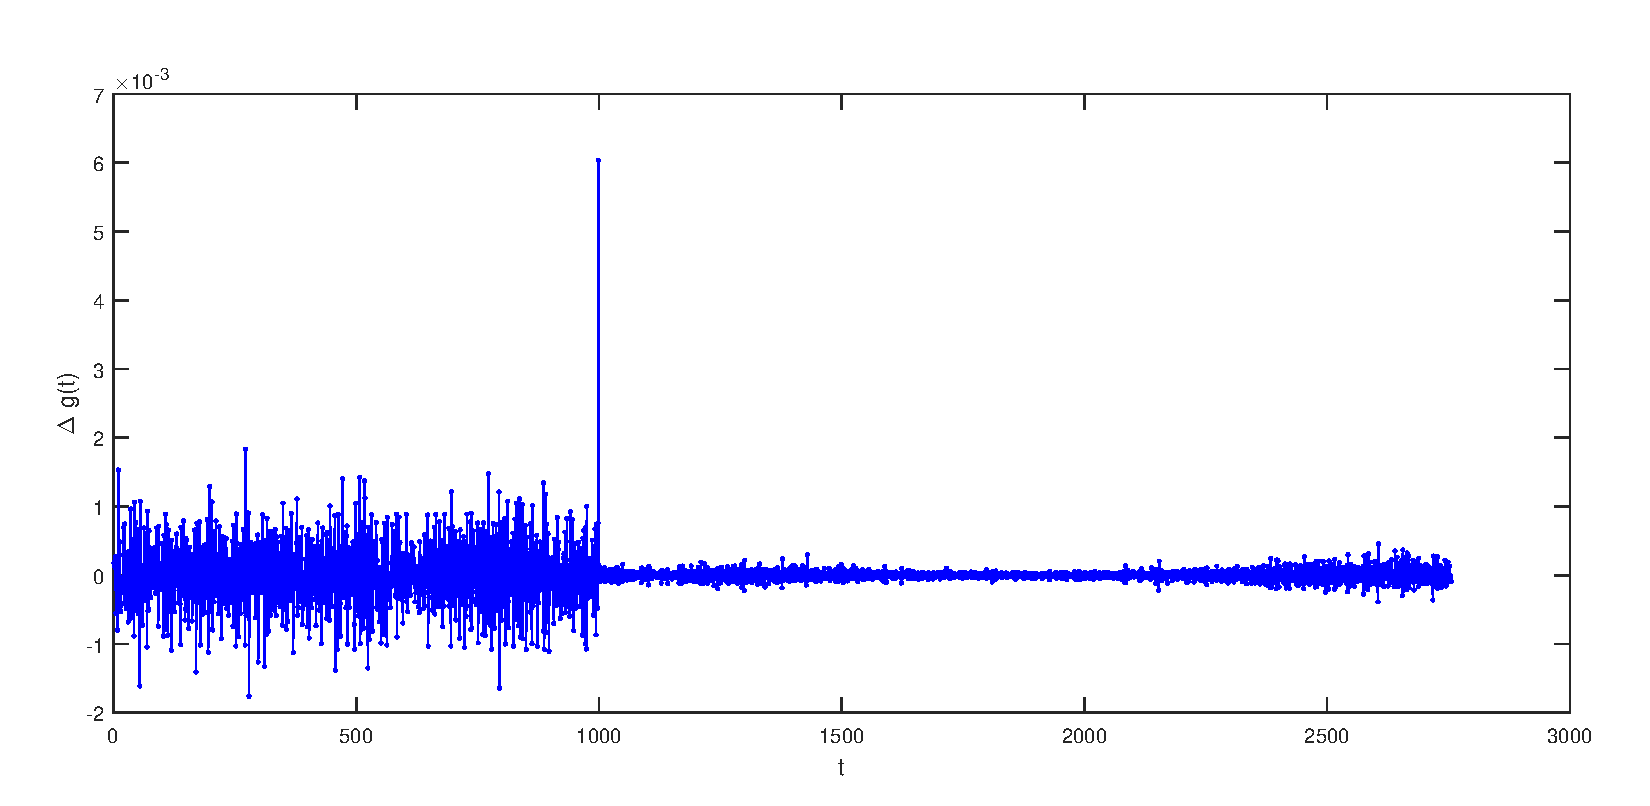
\includegraphics[width=12cm]{./pictures/Defocus/DEFOCUS_energy_detr}}
	\end{subfigure}
	\caption{Energia media del gradiente (a) e suo detrending (b) nel caso di una sfocatura}
	\label{fig:defocusPLOT}
\end{figure}
\begin{figure}[tb]
	\centering
	\begin{subfigure}[]
		{\label{fig:lumaDefocus} 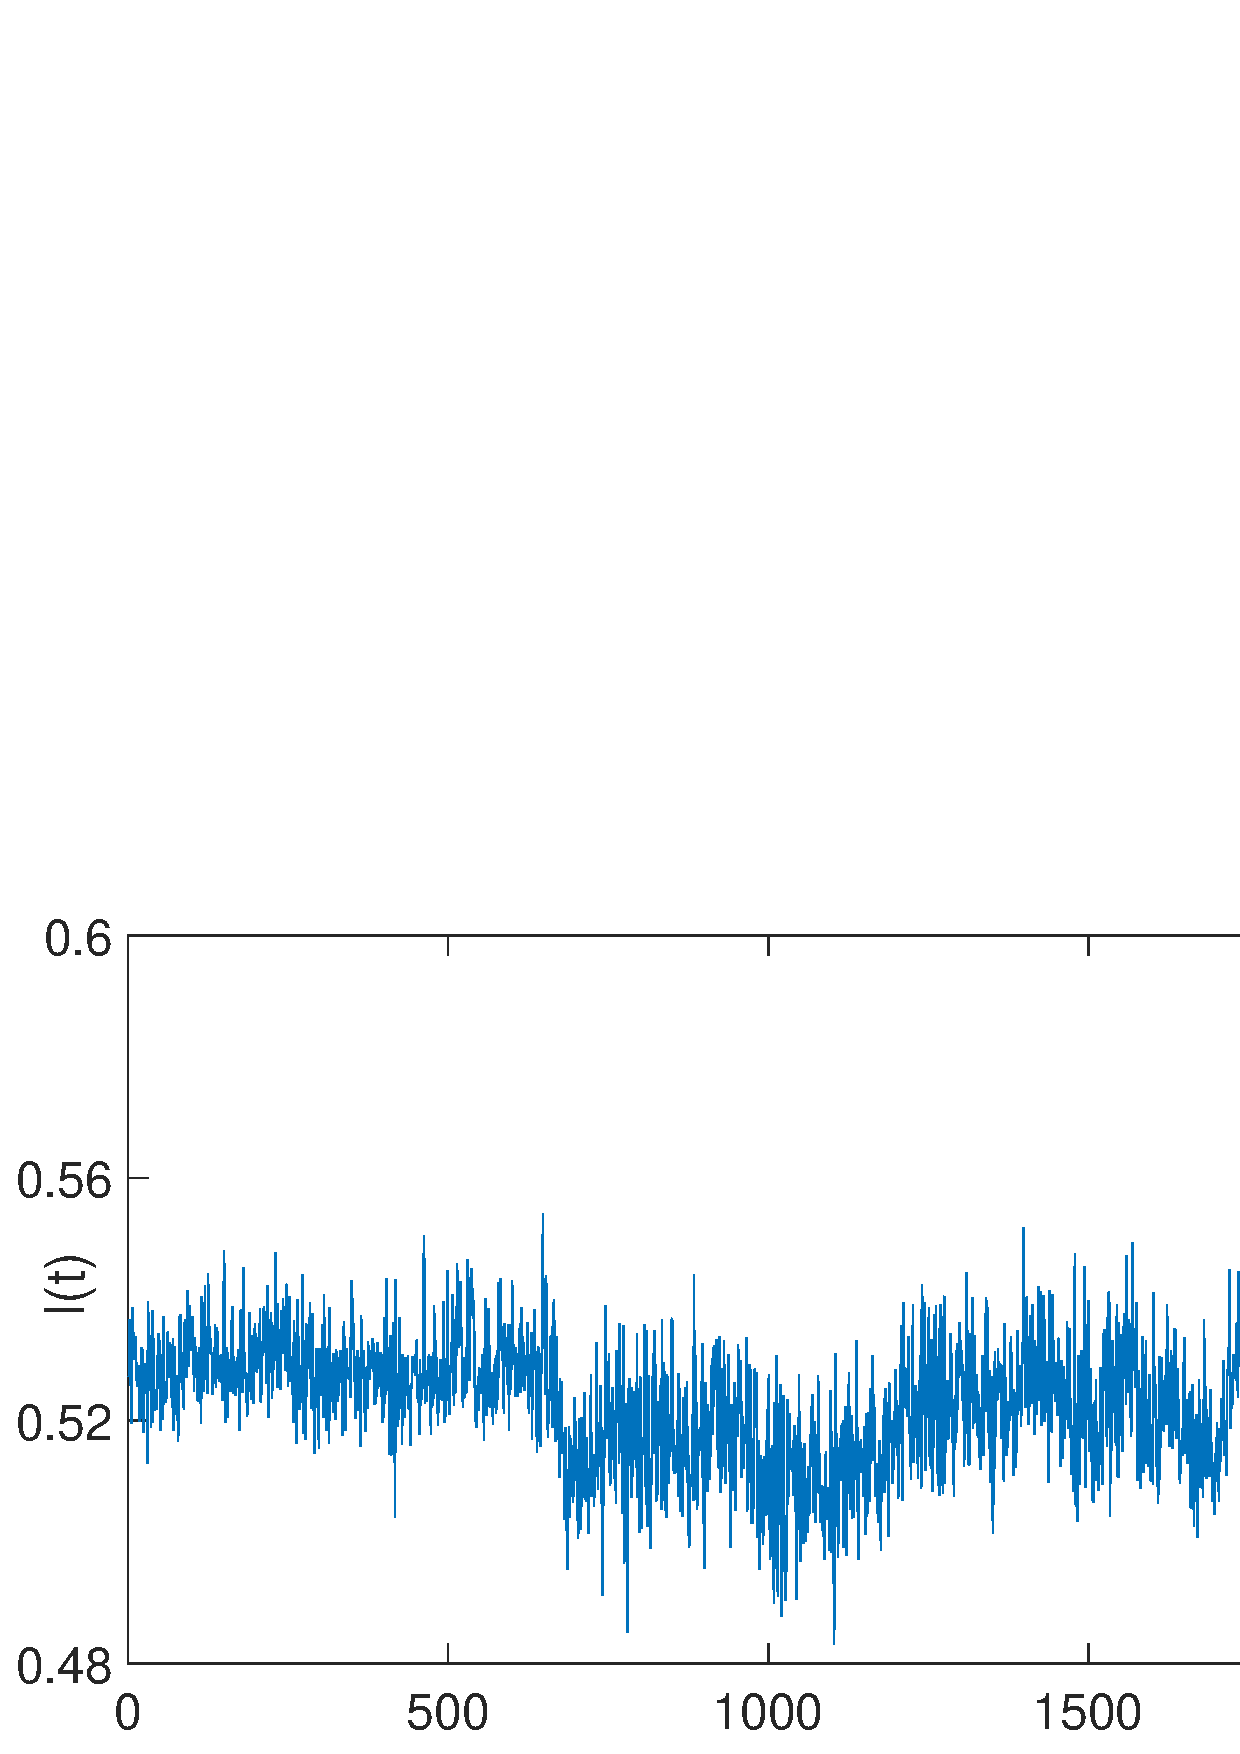
\includegraphics[width=12cm]{./pictures/Defocus/DEFOCUS_luma}}
	\end{subfigure}
	\begin{subfigure}[]
		{\label{fig:lumaDetrDefocus} 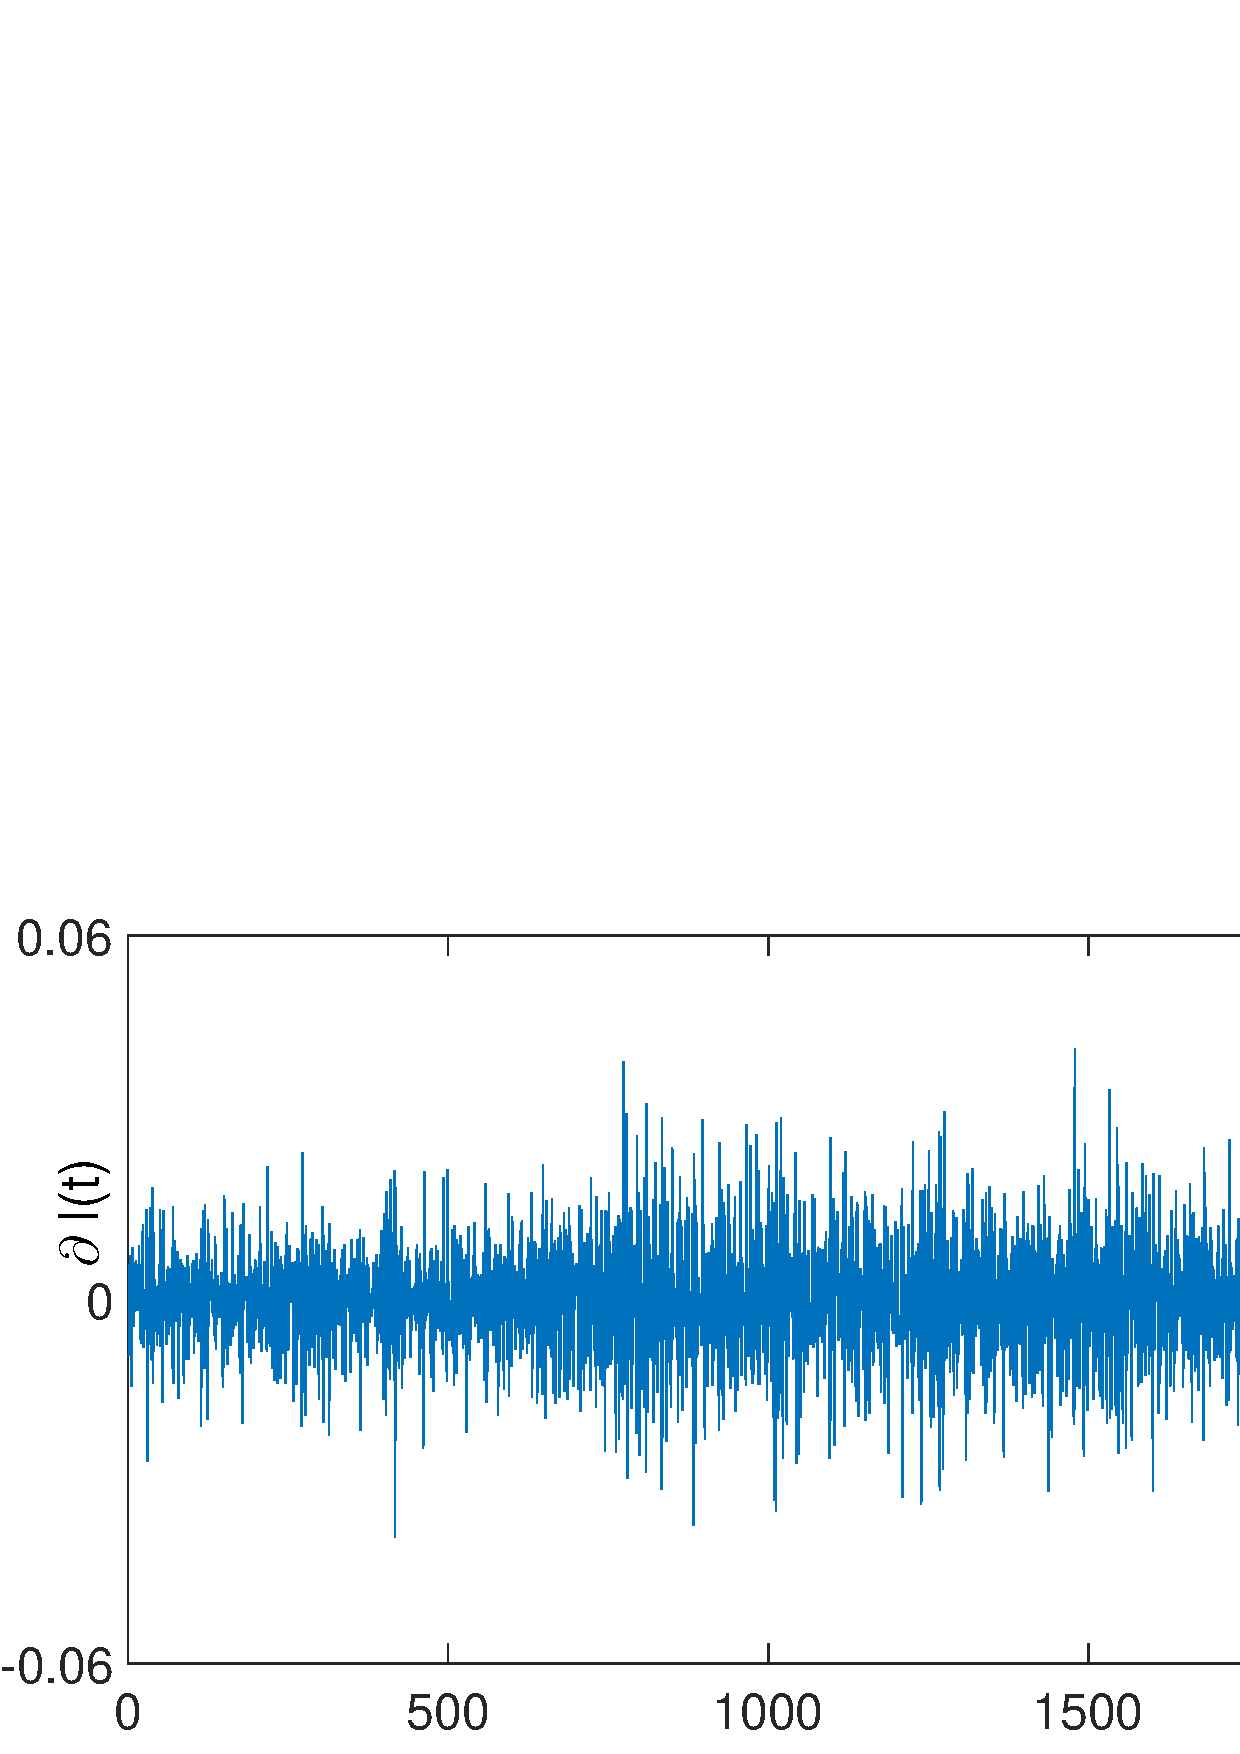
\includegraphics[width=12cm]{./pictures/Defocus/DEFOCUS_luma_detr}}
	\end{subfigure}
	\caption{Energia media della luma (a) e suo detrending (b) nel caso di una sfocatura}
	\label{fig:defocusDetrPLOt}
\end{figure}
\begin{figure}[tb]
	\centering
	\begin{subfigure}[]
		{\label{fig:energyDisplacement} 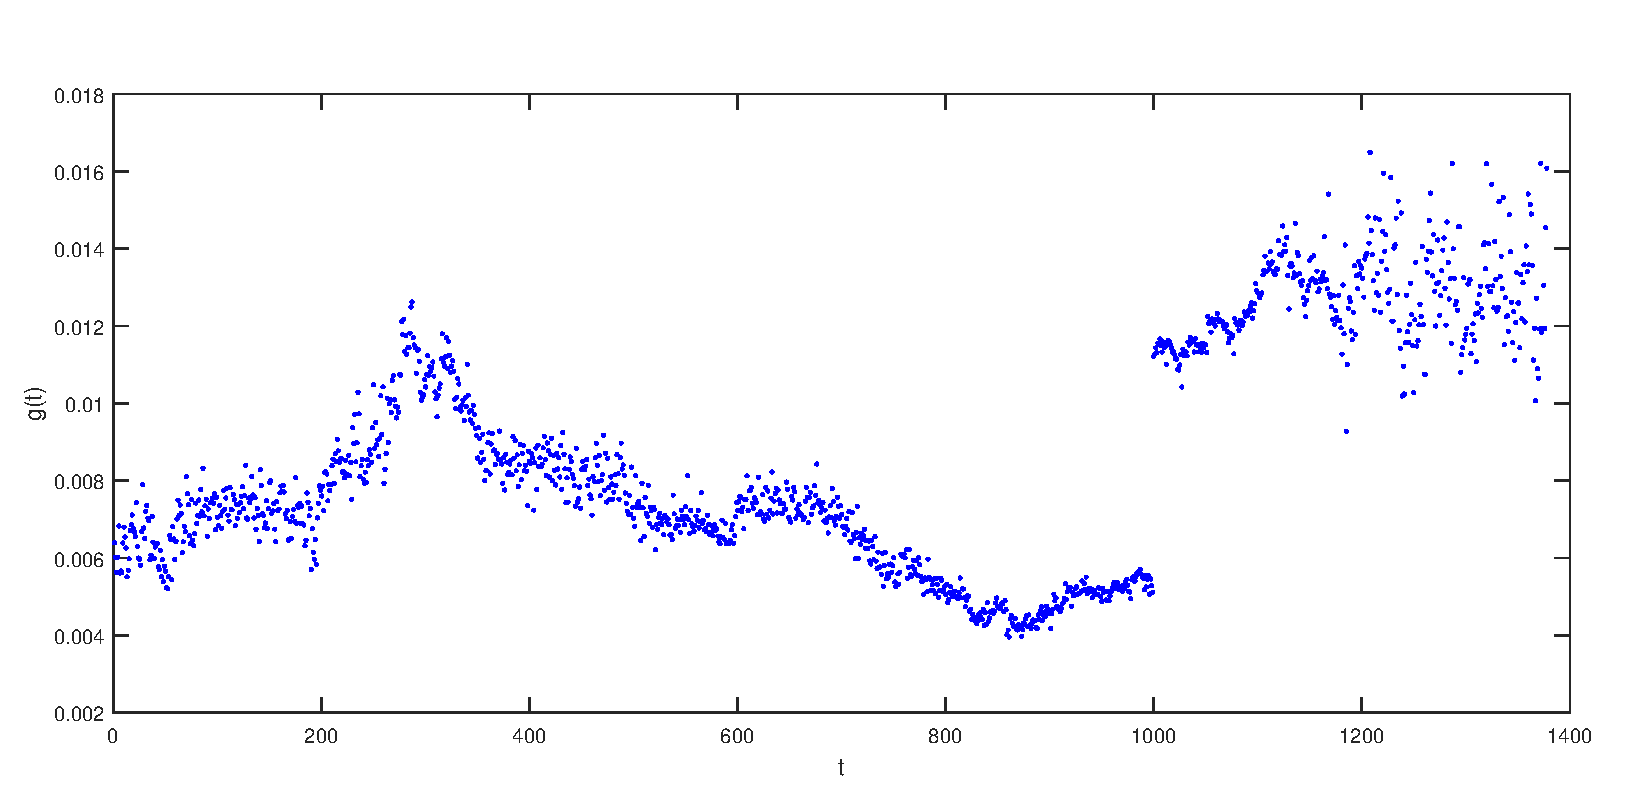
\includegraphics[width=12cm]{./pictures/Displacement/DISPLACEMENT_energy}}
	\end{subfigure}
	\begin{subfigure}[]
		{\label{fig:energyDetrDisplacement} 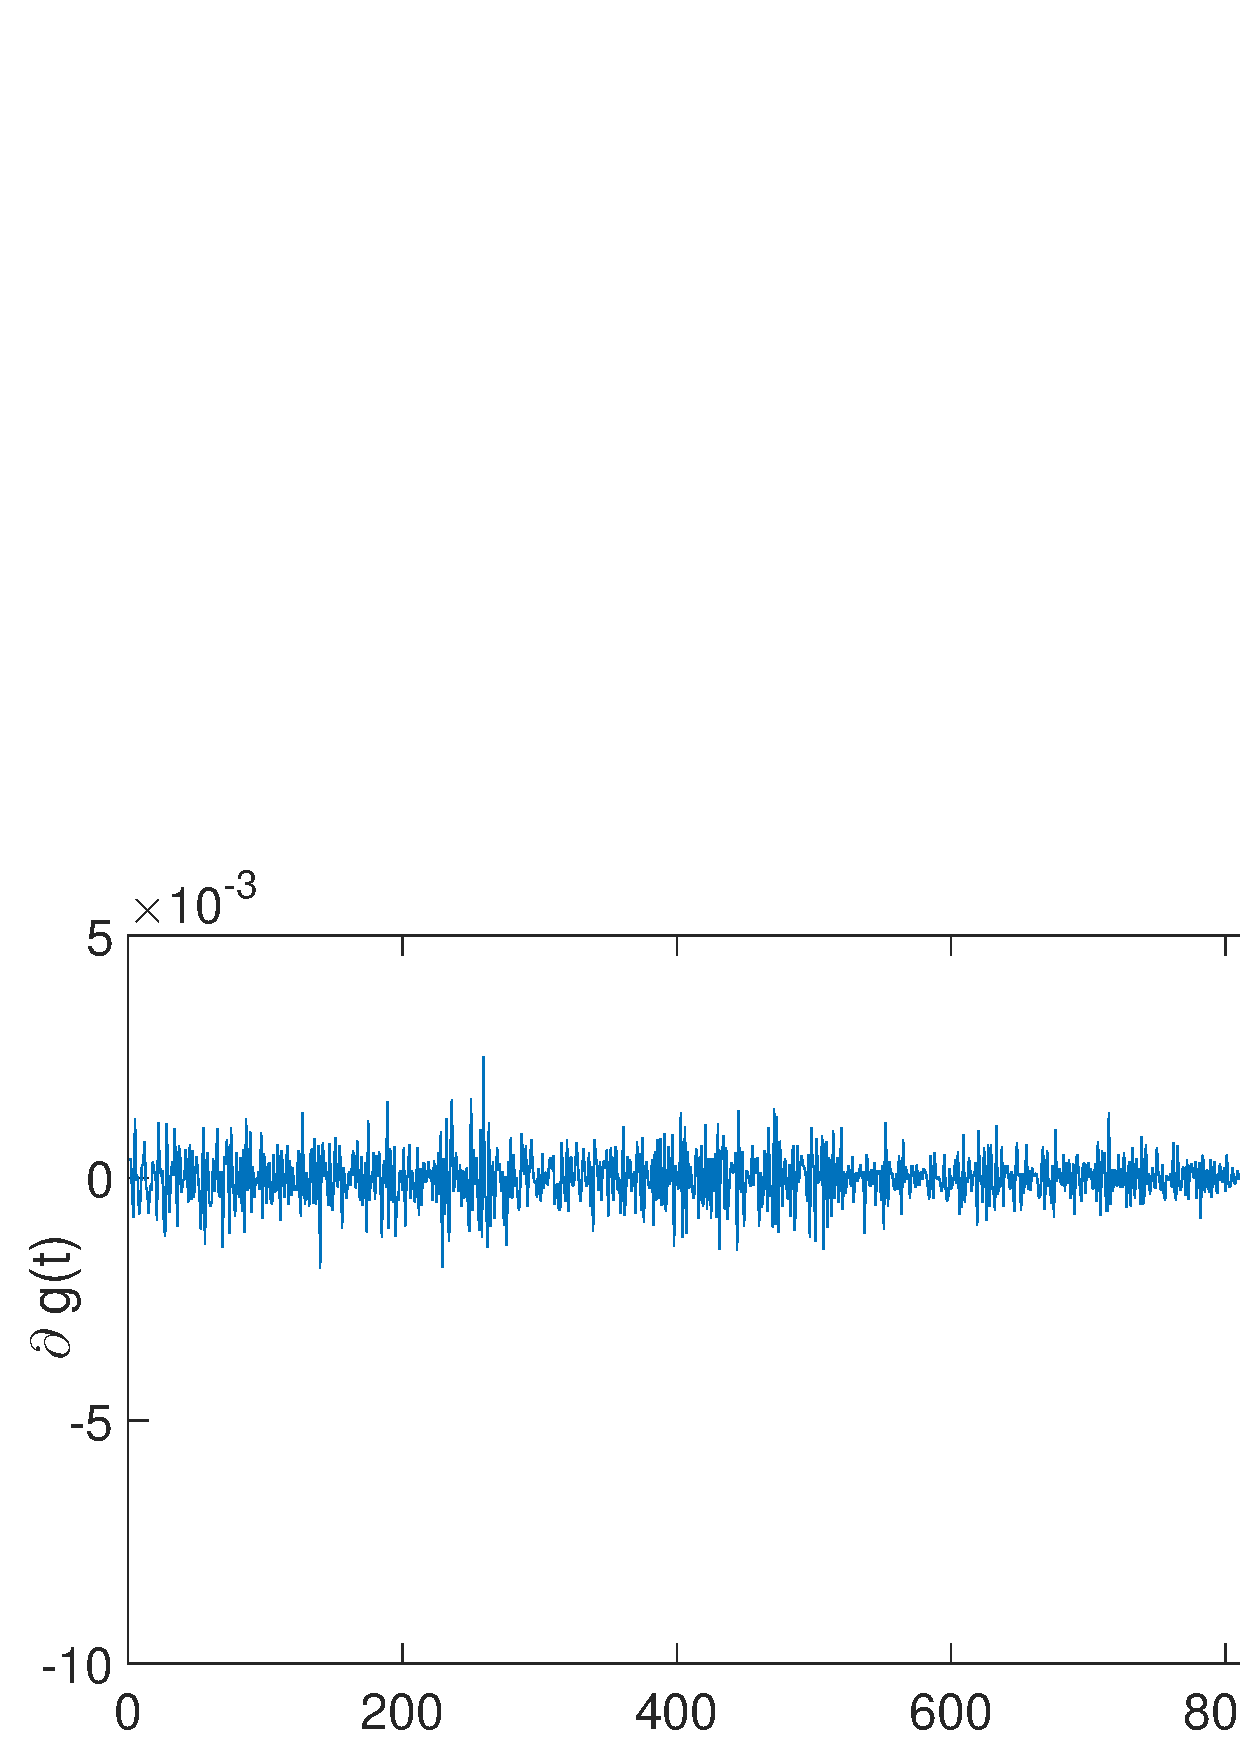
\includegraphics[width=12cm]{./pictures/Displacement/DISPLACEMENT_energy_detr}}
	\end{subfigure}
	\caption{Energia media del gradiente (a) e suo detrending (b) nel caso di uno spostamento della camera}
	\label{fig:displacementPLOT}
\end{figure}
\begin{figure}[tb]
	\centering
	\begin{subfigure}[]
		{\label{fig:lumaDisplacement} 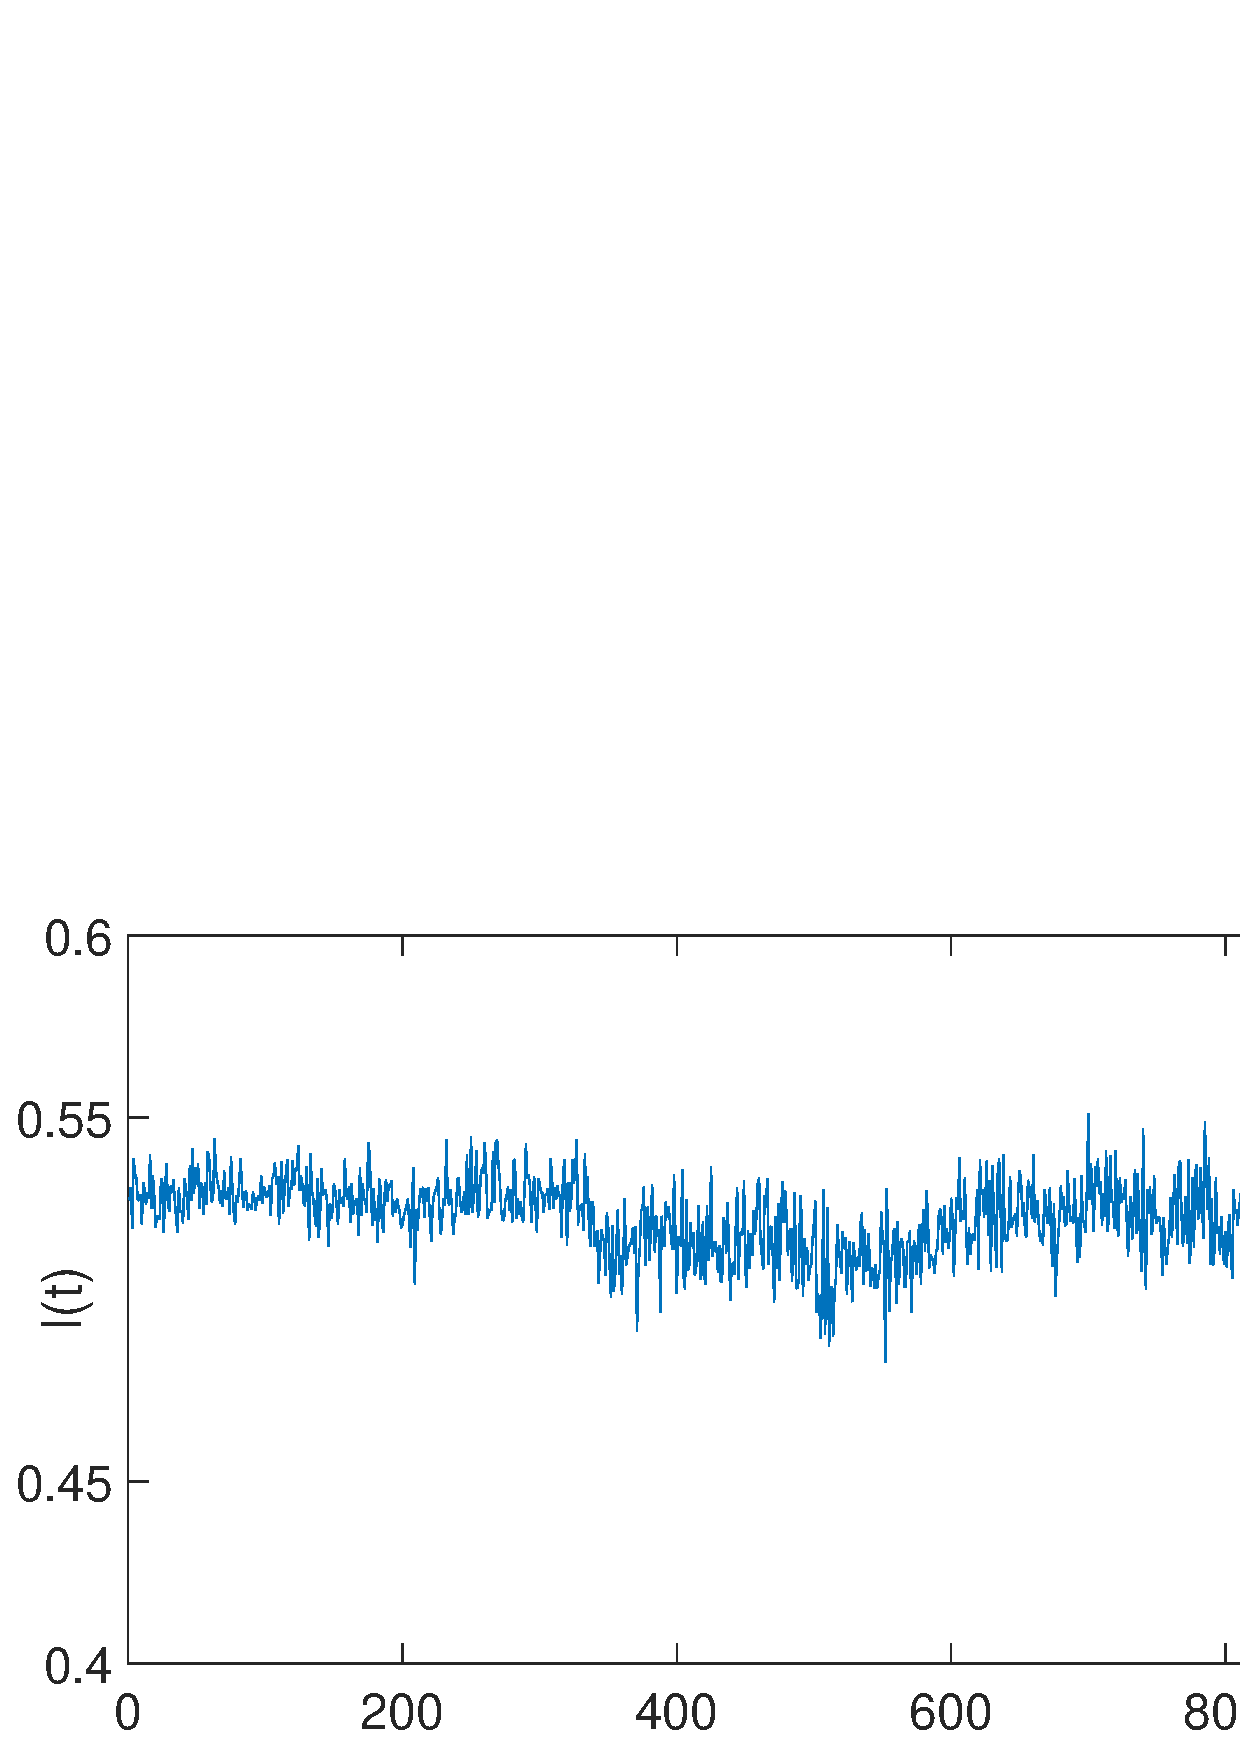
\includegraphics[width=12cm]{./pictures/Displacement/DISPLACEMENT_luma}}
	\end{subfigure}
	\begin{subfigure}[]
		{\label{fig:lumaDetrDisplacement} 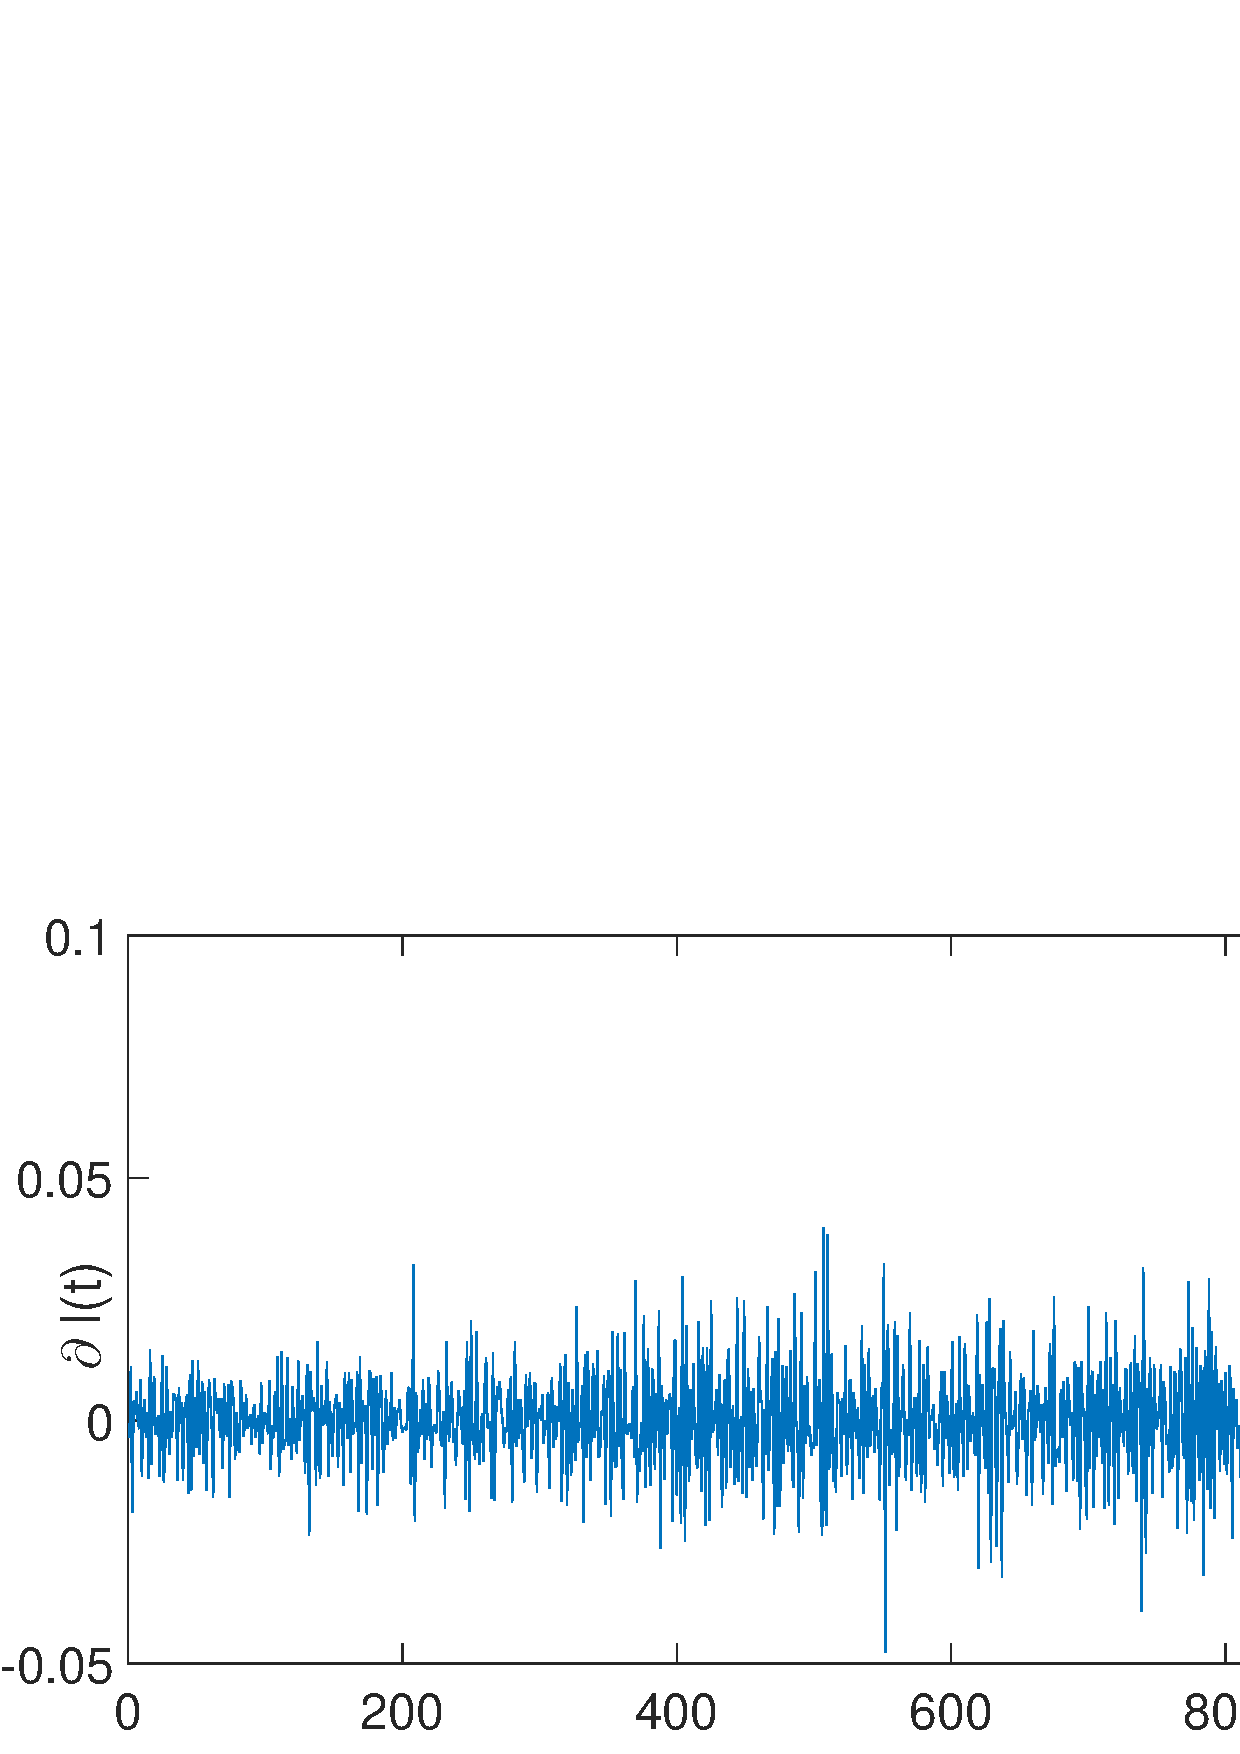
\includegraphics[width=12cm]{./pictures/Displacement/DISPLACEMENT_luma_detr}}
	\end{subfigure}
	\caption{Energia media della luma (a) e suo detrending (b) nel caso di uno spostamento della camera}
	\label{fig:displacementDetrPLOT}
\end{figure}
\begin{figure}[tb]
	\centering
	\begin{subfigure}[]{\label{fig:lumaDisplacementBRUTTO} 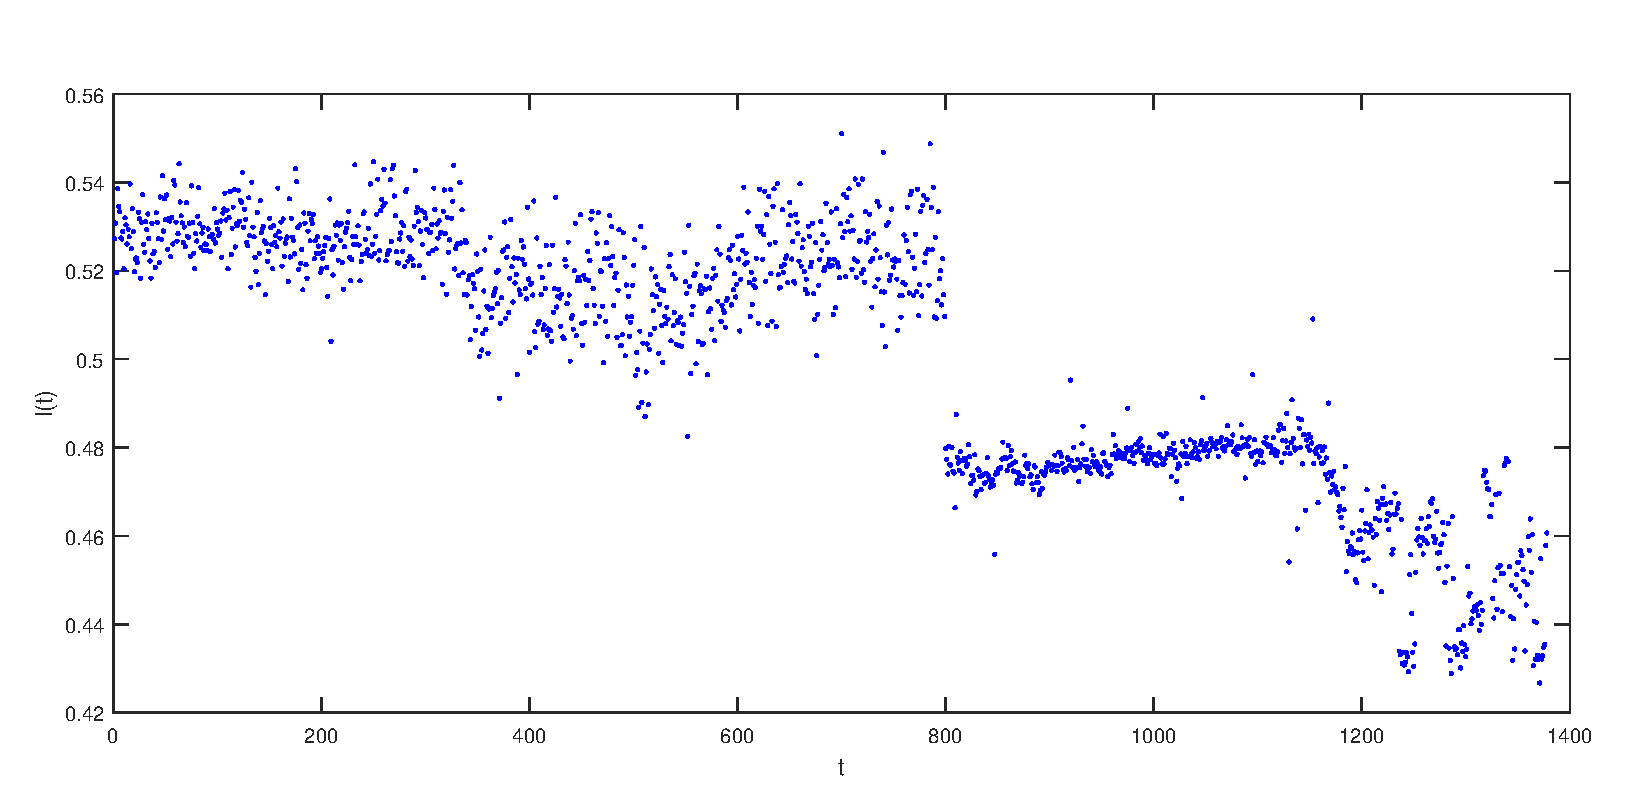
\includegraphics[width=12cm]{./pictures/DisplacementTOTALE/luma}}
	\end{subfigure}
	\begin{subfigure}[]
		{\label{fig:lumaDetrDisplacementBRUTTO} 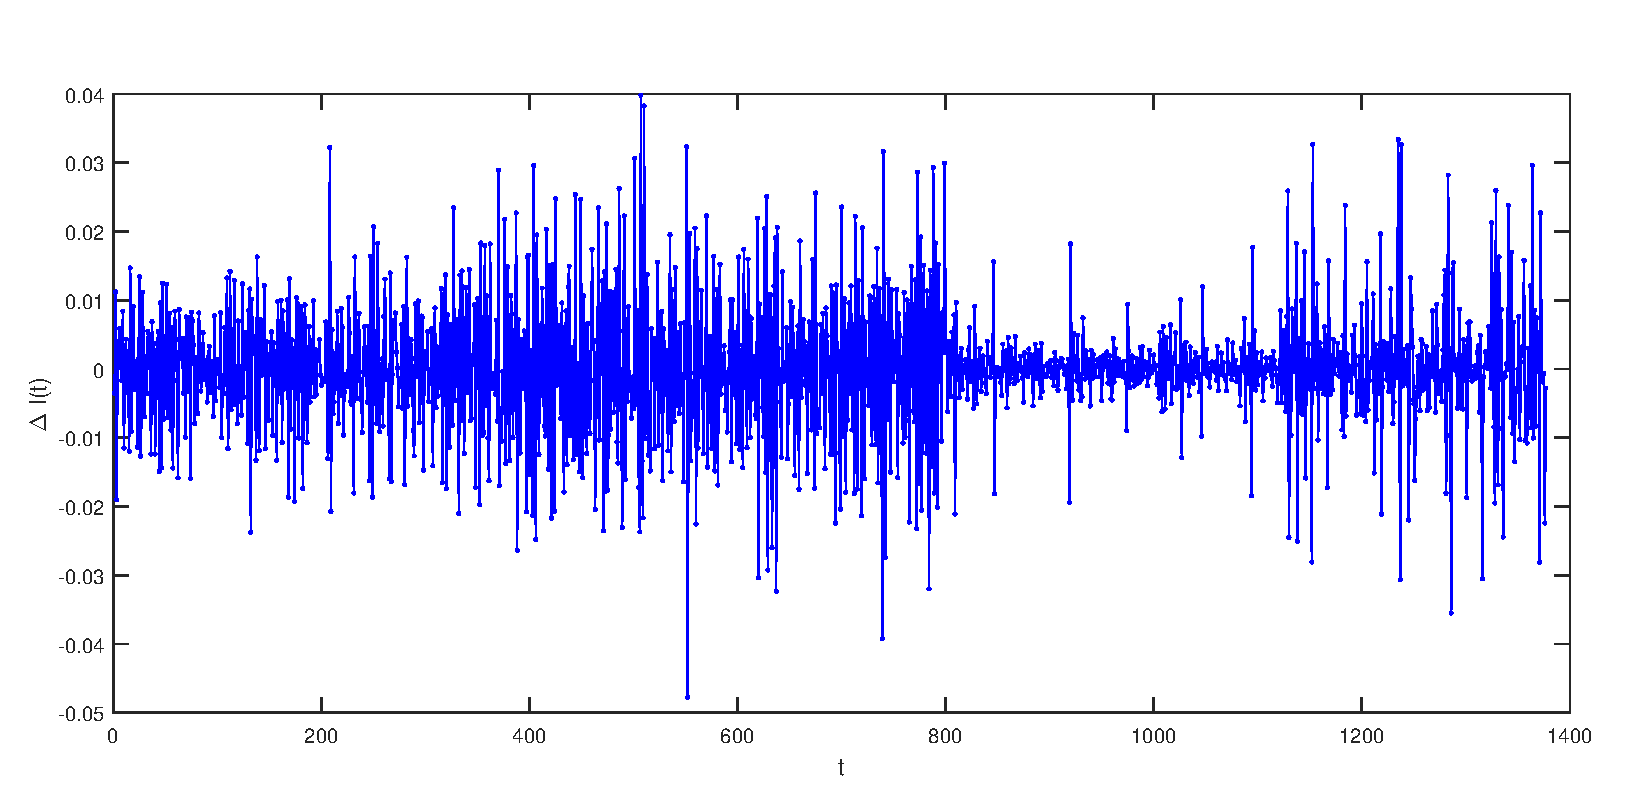
\includegraphics[width=12cm]{./pictures/DisplacementTOTALE/lumaDetr}}
	\end{subfigure}
	\caption{Esempio di sequenza dell'energia media della luma (a) e del suo detrending (b) con un displacement difficile da identificare}
	\label{fig:displacementBRUTTO}
\end{figure}
\begin{figure}[tb]
	\centering
	\subfigure[]{\label{fig:displacementORIGINALE1} 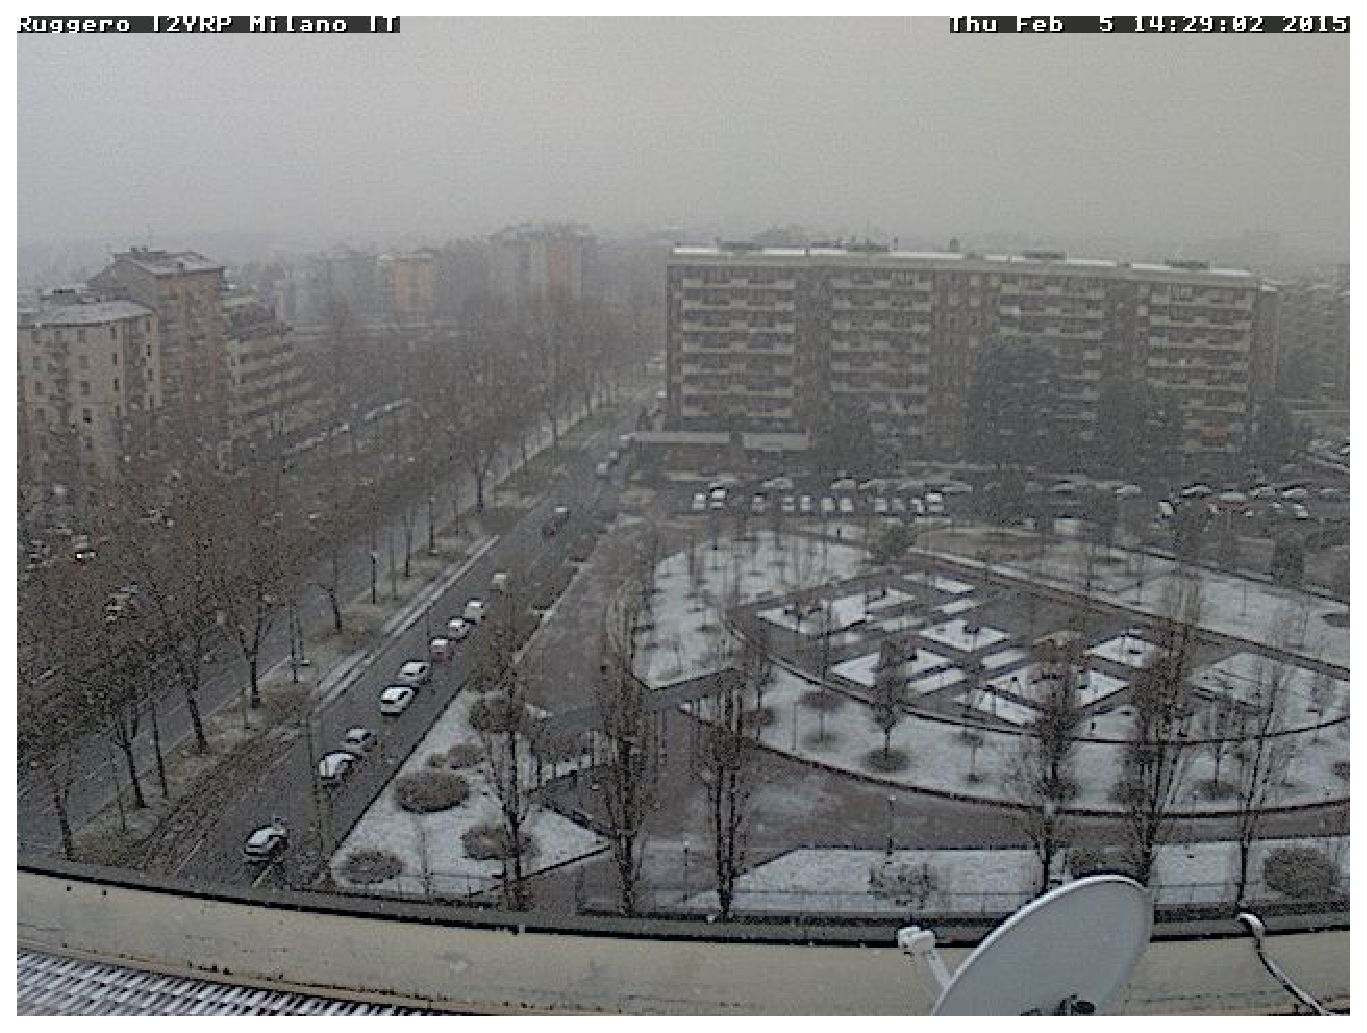
\includegraphics[width=6cm]{./pictures/testiORIGINALE}}
	\subfigure[]{\label{fig:displacementSPOSTATO1}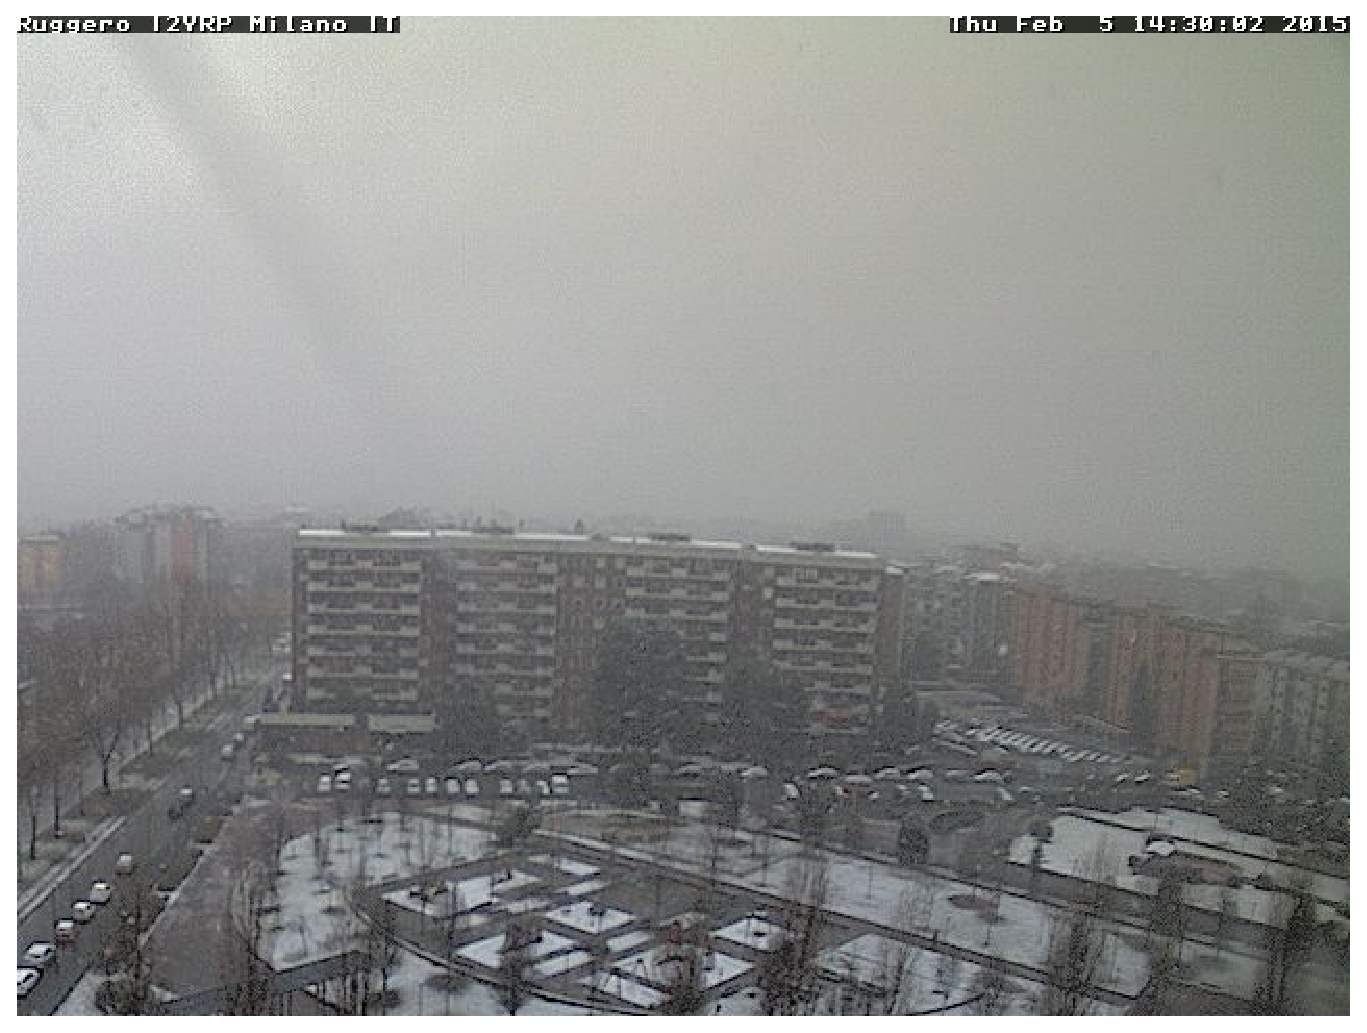
\includegraphics[width=6cm]{./pictures/testiDISPLACEMENT}}
	\caption{Esempio di spostamento della camera}
	\label{fig:testiDISPLACEMENT1}
\end{figure}
Questi fenomeni fanno s\`i che i nostri indicatori abbiano una dinamica \textit{difficilmente prevedibile} e che \textit{non siano stazionari}, come possiamo vedere negli esempi delle figure \ref{fig:energy} e \ref{fig:luma}.
Di conseguenza non \`e possibile applicare direttamente le tecniche di CDT come fatto in \cite{alippi2010detecting}. \\
Per eliminare le componenti in bassa frequenza possiamo fare un \textit{detrending} di ciascun segnale calcolando la \textit{differenza} tra l'indicatore all'istante corrente e quello precedente.
Nel caso dell'energia media del gradiente avremo
\begin{equation}
\label{eq:gradientDetr}
\Delta g_t = g_t - g_{t-1},
\end{equation}
mentre per l'energia media della luma avremo
\begin{equation}
\label{eq:lumaDetr}
\Delta l_t = l_t - l_{t -1}.
\end{equation}
Vediamo un esempio di come si comporta il detrending sui nostri indicatori nelle figure \ref{fig:energyDetr} e \ref{fig:lumaDetr}.  
Possiamo notare come le fluttuazioni in bassa frequenza vengano lavate via dal detrending, dato che in questo modo consideriamo solamente le differenze tra misure consecutive.\\
Come abbiamo detto prima, lo scopo del monitoraggio di questi indicatori \`e quello di individuare degli eventi di tampering.
Nelle figure \ref{fig:defocusPLOT} e \ref{fig:displacementPLOT} possiamo vedere il comportamento dell'energia media di luma e gradiente rispettivamente per un caso di sfocatura e per un caso di spostamento della camera.  
In particolare, in entrambi i casi l'evento di tampering avviene al frame $1000$\footnote{Il modo in cui sono stati ottenuti gli eventi di tampering \`e descritto nel Capitolo \ref{ProveSperimentali}}.
Il detrending di questi segnali \`e visualizzato nelle figure \ref{fig:defocusDetrPLOt} e \ref{fig:displacementDetrPLOT}.\\
\noindent Possiamo vedere come, in generale, l'evento di tampering sia associato a un brusco salto o a un crollo \textit{istantaneo} del valore di uno o entrambi gli indicatori.
Vanno notate alcune cose:
\begin{itemize}
	\item L'evento di sfocatura non si traduce in un cambiamento nell'energia media della luma.
	Questo avviene perch\'e questo tipo di tampering ha come effetto principale quello di rendere pi\`u morbide le differenze di intensit\`a tra i pixel dell'immagine, mantenendo comunque il valore medio della luma invariato.
	\item Facendo il detrending della sequenza abbiamo dei valori che oscillano attorno allo zero, un picco in corrispondenza dell'istante in cui avviene il tampering (figure \ref{fig:energyDetrDefocus}, \ref{fig:energyDetrDisplacement}, \ref{fig:lumaDetrDisplacement}) e infine altri valori che oscillano attorno allo zero.
	Questo \`e dato dal fatto che il detrending considera le differenze tra dati consecutivi e, quindi, la differenza maggiore si ha proprio nell'istante in cui inizia l'evento di tampering, mentre solitamente le differenze tra misure consecutive sono minime. 
	\item Questo fa s\`i che monitorare il detrending delle sequenze degli indicatori permetta di identificare pi\`u facilmente gli eventi di tampering rispetto ad analizzare la sequenza originale.
	Il risvolto della medaglia \`e che i cambiamenti \textit{persistenti}, come quelli che stiamo considerando noi, diventano dei cambiamenti \textit{istantanei}.
	\item Considerando l'evento di sfocatura, possiamo notare (Figura \ref{fig:energyDefocus}) come, in seguito all'evento, oltre ad aver un crollo istantaneo del valore dell'energia del gradiente, abbiamo anche un \textit{abbassamento della sua varianza}.
	Questo permette di utilizzare tecniche di monitoraggio sequenziale sull'energia del gradiente, con dei CDT sulla varianza, per identificare eventi di sfocatura.
\end{itemize}
In definitiva, \`e possibile identificare un evento di tampering andando a monitorare il detrending degli indicatori descritti dalla formule \eqref{eq:energyGradient} e \eqref{eq:energyLuma}.
Il monitoraggio pu\`o essere fatto con tecniche a \textit{basso carico computazionale}: infatti \`e possibile utilizzare semplicemente delle soglie in modo da individuare il picco nel detrending dovuto all'evento di tampering.
In particolare possiamo monitorare l'energia media del gradiente per individuare eventi di sfocatura, e l'energia media della luma per individuare eventi di spostamento della camera.
Inoltre, per rendere pi\`u robusta l'identificazione di sfocature, \`e possibile usare un test sequenziale sull'energia media del gradiente in grado di individuare dei cambiamenti nella varianza.\\
Dobbiamo fare un'ultima considerazione sullo spostamento della camera.
Ci possono essere dei casi in cui l'evento \`e difficilmente individuabile monitorando la scena nella sua totalit\`a.
Un esempio \`e illustrato nella Figura \ref{fig:displacementBRUTTO}, dove vediamo un caso di spostamento della camera che avviene al frame $800$.
Questo evento, per\`o, non si traduce, nel detrending del segnale, in un picco che si eleva rispetto agli altri, come nel caso della Figura \ref{fig:lumaDetrDisplacement}.
Questo problema capita perch\'e stiamo monitorando l'energia media della luma calcolata sulla \textit{totalit\`a} della scena.
Possiamo avere situazioni, come nel caso della Figura \ref{fig:displacementBRUTTO}, in cui lo spostamento della camera non determina un cambiamento sostanziale nella luminosit\`a media della scena.\\
Questo problema viene meno se consideriamo il contributo dell'energia della luma mediato non sulla totalit\`a della scena, bens\`i su \textit{regioni} specifiche analizzate separatamente.
Infatti, se consideriamo un'area particolare della scena, come ad esempio quella occupata dal palazzo nella Figura \ref{fig:displacementORIGINALE1}, durante uno spostamento della camera la variazione della luma mediata solo sui pixel appartenenti a quella regione sar\`a pi\`u marcata rispetto a quella della luminosit\`a mediata su tutta l'immagine.
%Nella Figura  \ref{fig:testiDISPLACEMENT1}, tra il frame \ref{fig:displacementORIGINALE1} e il frame \ref{fig:displacementSPOSTATO1}, l'area occupata dal palazzo cambia il suo contenuto riprendendo un pezzo di cielo.
Abbiamo deciso, quindi, di inserire una fase di \textit{segmentazione} in cui vengono estratte le regioni della scena che la camera deve inquadrare.
 \begin{figure}[tb]
 	\centering
 	\subfigure[]{\label{fig:testiSCENA} 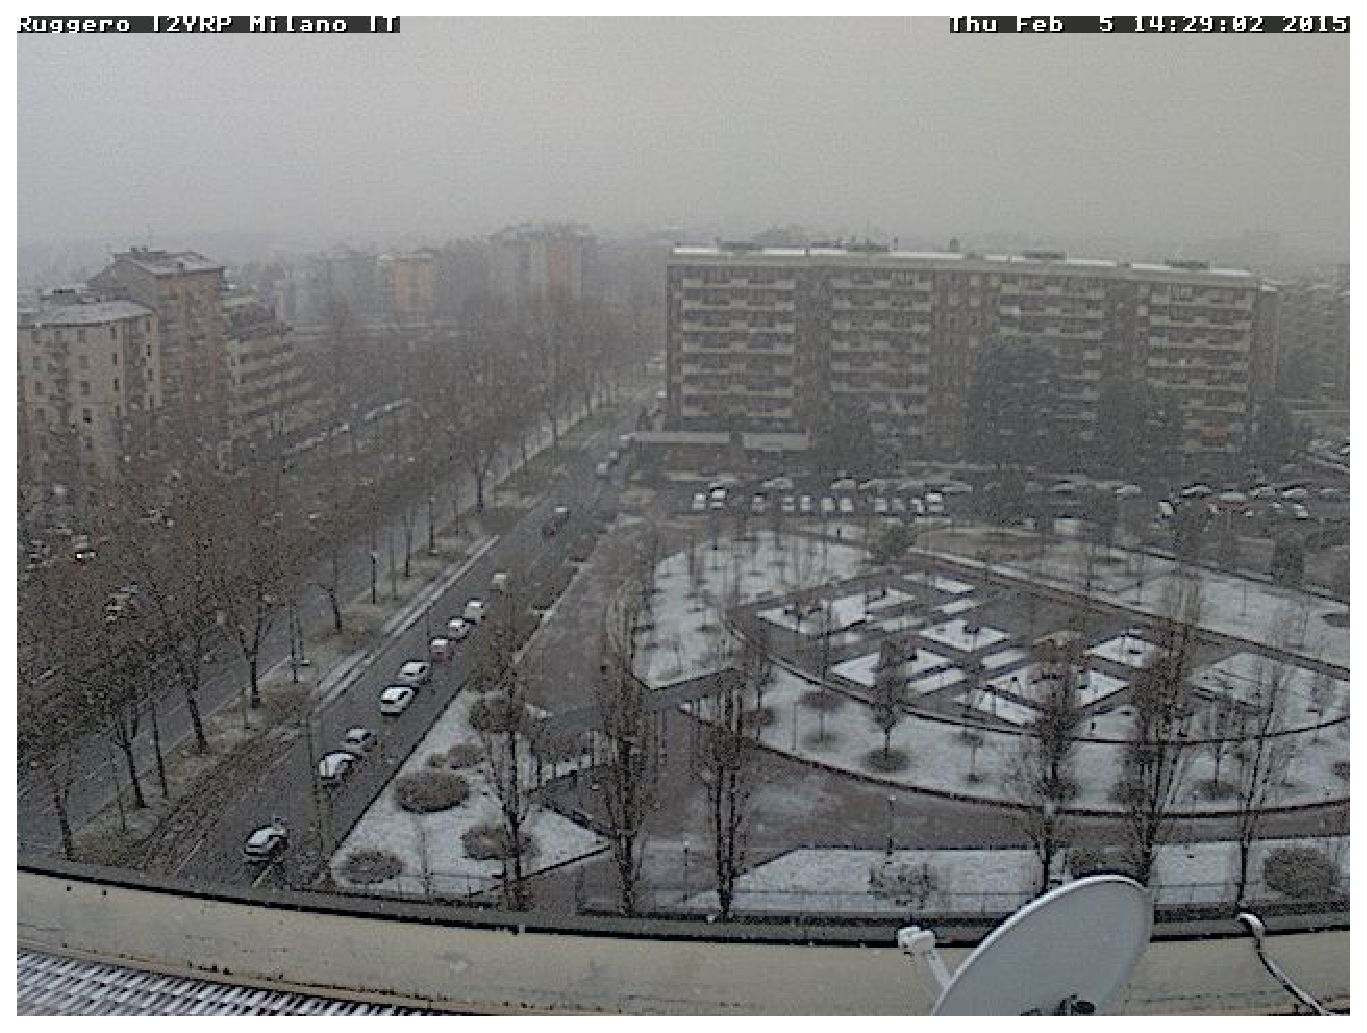
\includegraphics[width=6cm]{./pictures/testiORIGINALE}}
 	\subfigure[]{\label{fig:testiMAPPA}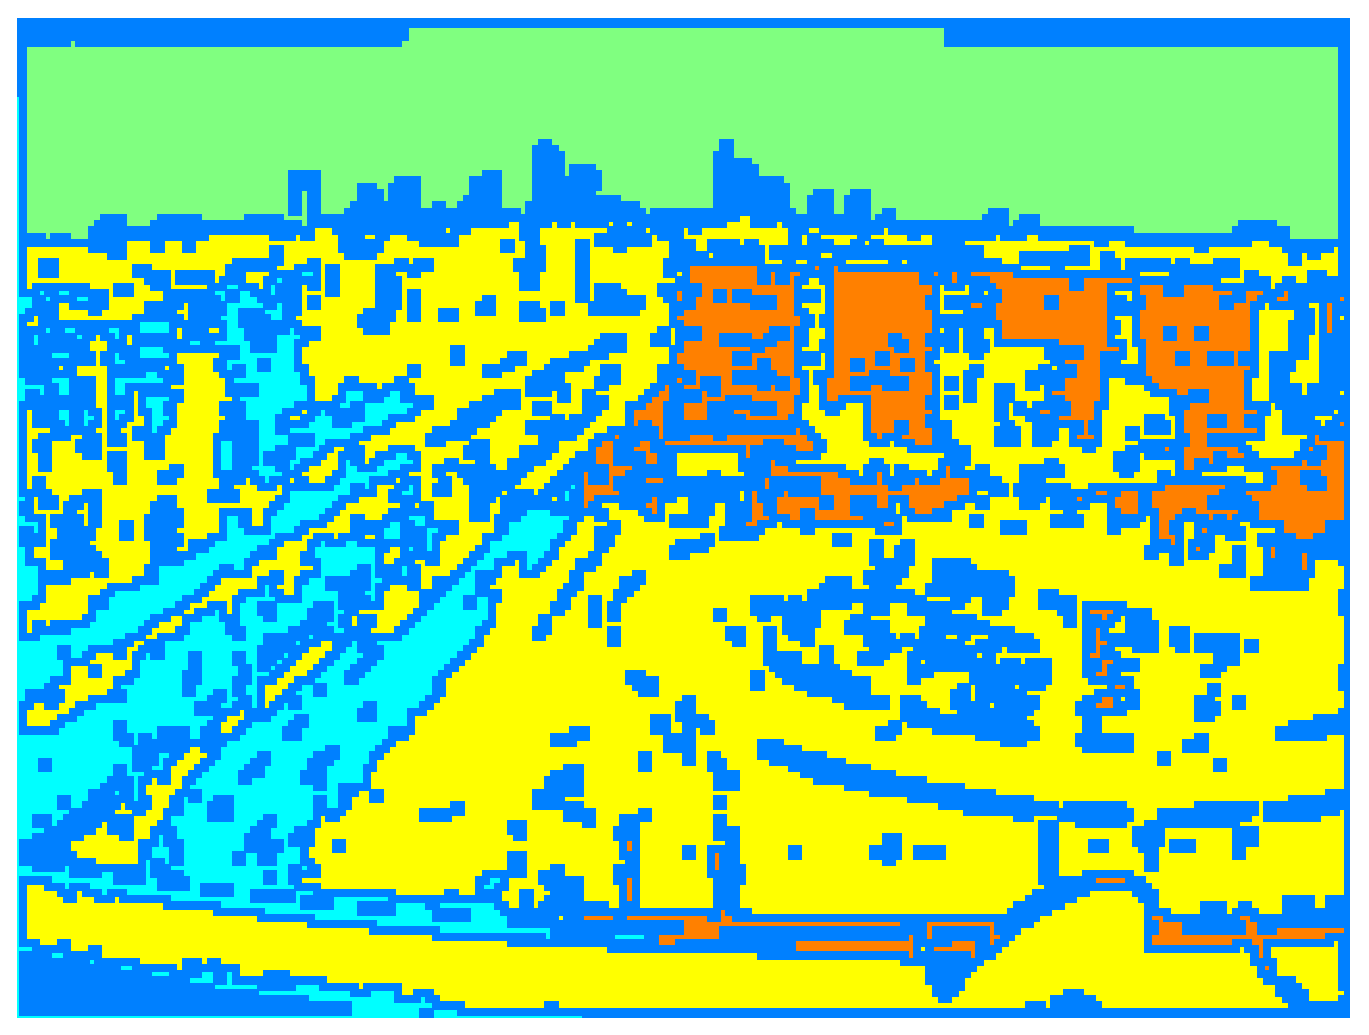
\includegraphics[width=6cm]{./pictures/map}}
 	\caption{Esempio di segmentazione della scena}
 	\label{fig:testiSEGMENTAZIONE}
 \end{figure}
Un esempio \`e illustrato nella Figura \ref{fig:testiSEGMENTAZIONE}. 
Nel Paragrafo \ref{segmentazione} vedremo in dettaglio come vengono estratte le regioni dalla scena.
\section{Algoritmo di identificazione di sfocature e di spostamenti della camera}
\label{monitoraggio}
In base alle considerazioni fatte nel Paragrafo \ref{indicatori} possiamo dividere l'algoritmo di tampering detection in due \textit{thread}:
il primo in grado di individuare la presenza di sfocature all'interno di un'immagine, il secondo lo spostamento della camera.
In particolare la presenza di sfocature pu\`o essere identificata monitorando l'energia media del gradiente (Formula \eqref{eq:energyGradient}), mentre l'evento di spostamento della camera pu\`o essere identificato monitorando l'energia media della luma (Formula \eqref{eq:energyLuma}).\\
Nel corso di questo paragrafo illustriamo come sono state sviluppate le due tecniche.
\subsection{Identificazione delle sfocature}
L'Algoritmo \ref{alg:DEFOCUS} mostra il funzionamento, ad alto livello, dell'algoritmo per identificare la presenza di sfocature nei frame.
%\IncMargin{0.1em}
%\vspace{-0.2cm}
\begin{algorithm}[t]
	% \SetAlgoNoLine
	\LinesNumbered
	\SetAlgoNlRelativeSize{0}
	\SetNlSty{small}{}{.}
	\textbf{Configurazione}:\\
	\lnl{DEF-Tr1} \For{$t=1,\dots,T_{training}$}
	{	\lnl{DEF-Tr2} Estraggo il frame $z_t$ \\
		\lnl{DEF-Tr3} Calcolo $g_t$, $\Delta g_t$ \\
	}
	\lnl{DEF-Tr4} Definisco le soglie $Th_{min}^g$ e $Th_{max}^g$\\
	\lnl{DEF-Tr5} Definisco i parametri per il CDT sulla varianza di $g_t$\\
	\textbf{Fase operativa}:\\
	\lnl{DEF-Test1} \For{$t=T_{training},\dots,\infty$}{
		\lnl{DEF-Test2} Estraggo il frame $z_t$ \\
		\lnl{DEF-Test3} Calcolo $g_t$, $\Delta g_t$\\
		\lnl{DEF-Test4} \If{$\Delta g_t < Th_{min}^g \vee \Delta g_t > Th_{max}^g $}{
			\lnl{DEF-Test5} $z_t$ \`e un frame in cui \`e avvenuto una sfocatura\\
		}
		\lnl{DEF-Test8} \If{CDT identifica un cambiamento in $g_t$}{
			\lnl{DEF-Test9} $z_t$ \`e un frame in cui \`e avvenuto uno spostamento della camera\\
		}
	}   
	\caption{Algoritmo di identificazione di sfocature}
	\label{alg:DEFOCUS}
\end{algorithm}
Dato che la sfocatura causa un crollo dell'energia media del gradiente e anche della sua varianza, \`e possibile lanciare due monitoraggi in grado di identificare ciascuno di questi cambiamenti.\\
Il primo monitoraggio prevede un'analisi del detrending dell'energia media del gradiente, usando le Formule \eqref{eq:energyGradient} e \eqref{eq:gradientDetr}, in modo da identificare il picco dovuto al cambiamento (si veda la Figura \ref{fig:defocusPLOT}).
L'identificazione viene fatta attraverso la definizione di due \textit{soglie}, calcolate facendo riferimento alle prime $T_{training}$ osservazioni, ritenute prive di tampering.
Tale sequenza prende il nome di \textit{training set}.
Le due soglie $Th_{min}^g$ e $Th_{max}^g$ vengono calcolate nel seguente modo:
\begin{equation}
\label{eq:soglieGradiente}
\begin{array}{rcl}
Th_{min}^g & = & \mu_{\Delta g} -\Gamma \sigma_{\Delta g}\\
Th_{max}^g & = & \mu_{\Delta g} + \Gamma \sigma_{\Delta g}
\end{array},
\end{equation}
dove $\mu_{\Delta g}$ indica il valore medio delle osservazioni del training set
\begin{equation}
	\mu_{\Delta g}  = \frac{\sum_{t = 1}^{T_{training}} \Delta g_t}{T_{training}}, \nonumber
\end{equation}
$\sigma_{\Delta g}$ indica la deviazione standard delle osservazioni del training set
\begin{equation}
\sigma_{\Delta g}  = \sqrt{\frac{1}{T_{training}-1}\sum_{t=1}^{T_{training}}\left(\Delta g_t - \mu_{\Delta g}\right)^2} \nonumber
\end{equation}
e $\Gamma>1$ \`e un parametro moltiplicativo ottenuto sperimentalmente\footnote{Per maggiori dettagli si rimanda al Capitolo \ref{ProveSperimentali}}.\\
Le soglie definite nella Formula \eqref{eq:soglieGradiente} forniscono un limite superiore e uno inferiore ai valori di $\{\Delta g_t\}$ ammissibili.
Qualsiasi valore al di sotto di $Th_{min}$ o al di sopra di $Th_{max}$ viene considerato come un evento di sfocatura.\\ 
Oltre all'analisi sul detrending \`e possibile fare un monitoraggio sequenziale sulla varianza di $\{g_t\}$: infatti, come abbiamo visto nel paragrafo \ref{comportamento}, la presenza di una sfocatura comporta una diminuzione della varianza di questa sequenza.
Il monitoraggio sequenziale viene fatto utilizzando un CDT basato su ICI-rule\footnote{Lo schema di funzionamento del CDT basato su ICI-rule \`e spiegato nel Paragrafo \ref{cdt}.} sulla varianza di $\{g_t\}$, usando il training set per configurare i suoi parametri.


\subsection{Identificazione degli spostamenti della camera}
\label{monitoraggioDISPL}
L'Algoritmo \ref{alg:DISPL} mostra il funzionamento, ad alto livello, dell'algoritmo per identificare un evento di spostamento della camera.\\
\begin{algorithm}[t]
	% \SetAlgoNoLine
	\LinesNumbered
	\SetAlgoNlRelativeSize{0}
	\SetNlSty{small}{}{.}
	\textbf{Configurazione}:\\
	\lnl{DISPL-Tr1} Estraggo le regioni $\{R_k\}, k=1,\dots,K$  \\
	\lnl{DISPL-Tr2} \For{$t=1,\dots,T_{training}$}
	{	\lnl{DISPL-Tr3} Estraggo il frame $z_t$ \\
		\lnl{DISPL-Tr4} \For{$k=1,\dots,K$}{
			\lnl{DISPL-Tr5} Calcolo $l_t^k$, $\Delta l_t^k$ per la regione $R_k$\\
		}
	}
	\lnl{DISPL-Tr6} \For{$k=1,\dots,K$}{
		\lnl{DISPL-Tr7} Definisco le soglie $Th_{min}^k$ e $Th_{max}^k$\\
	}
	\textbf{Fase operativa}:\\
	\lnl{DISPL-Test1} \For{$t=T_{training},\dots,\infty$}{
		\lnl{DISPL-Test2} Estraggo il frame $z_t$ \\
		\lnl{DISPL-Test3} $n = 0$ \\
		\lnl{DISPL-Test4} \For{$k=1,\dots,K$}{
			\lnl{DISPL-Test5} Calcolo $l_t^k$, $\Delta l_t^k$ per la regione $R_k$\\
			\lnl{DISPL-Test6} \If{$\Delta l_t^k < Th_{min}^k \vee \Delta l_t^k > Th_{max}^k $}{
				\lnl{DISPL-Test7} $n=n+1$\\
			}
		}
		\lnl{DISPL-Test8} \If{$n\geq K-1$}{
			\lnl{DISPL-Test9} $z_t$ \`e un frame in cui \`e avvenuto uno spostamento della camera\\
		}
	}   
	\caption{Algoritmo di identificazione di spostamenti della camera}
	\label{alg:DISPL}
\end{algorithm}
Una prima fase dell'algoritmo consiste nella \textit{partizione} della scena inquadrata dalla camera in un insieme di regioni $\{R_k\}, k=1,\dots,K$.
Il metodo con cui vengono estratte queste regioni verr\`a analizzato in dettaglio nel paragrafo \ref{segmentazione}. \\
L'analisi che viene fatta \`e simile a quella vista nel monitoraggio del detrending dell'energia del gradiente:
in questo caso l'analisi \`e fatta in maniera indipendente per ciascuna regione $R_k$, calcolando l'energia della luma \textit{mediata per i pixel appartenenti alla regione}:
\begin{equation}
	\label{eq:lumaRegions}
	\begin{array}{rl}
	l_t^k&  =  \mathcal{L}^k[z_t] = \frac{\sum_{\mathcal{X}} z_t(x) }{|\mathcal{X}|_{R_k}}\\
	\Delta l_t^k & = l_t^k-l_{t-1}^k 
	\end{array},
\end{equation}
dove abbiamo indicato con $|\mathcal{X}|_{R_k}$ il numero totale dei pixel appartenenti alla regione $R_k$.\\
L'identificazione viene fatta attraverso la definizione di due \textit{soglie}, calcolate facendo riferimento alle prime $T_{training}$ osservazioni, ritenute prive di tampering.
Le due soglie $Th_{min}^k$ e $Th_{max}^k$ vengono calcolate per ciascuna regione nel seguente modo:
\begin{equation}
\label{eq:soglieLuma}
\begin{array}{rcl}
Th_{min}^k & = & \mu_{\Delta l^k} -\Gamma \sigma_{\Delta l^k}\\
Th_{max}^k & = & \mu_{\Delta l^k} + \Gamma \sigma_{\Delta l^k}
\end{array},
\end{equation}
dove $\mu_{\Delta l^k}$ indica il valore medio delle osservazioni del training set
\begin{equation}
\mu_{\Delta l^k}  = \frac{\sum_{t = 1}^{T_{training}} \Delta l_t^k}{T_{training}}, \nonumber
\end{equation}
$\sigma_{\Delta l^k}$ indica la deviazione standard delle osservazioni del training set
\begin{equation}
\sigma_{\Delta l^k}  = \sqrt{\frac{1}{T_{training}-1}\sum_{t=1}^{T_{training}}\left(\Delta l_t^k - \mu_{\Delta l^k}\right)^2} \nonumber
\end{equation}
e $\Gamma>1$ \`e un parametro moltiplicativo ottenuto sperimentalmente.\\
Le soglie definite nella Formula \eqref{eq:soglieLuma} forniscono un limite superiore e uno inferiore ai valori di $\{\Delta l_t^k\}$ ammissibili.\\
Dato che l'evento di spostamento della camera viene inteso come un cambiamento globale dell'immagine, ci aspettiamo che tale cambiamento sia percepibile in tutte le regioni contemporaneamente. 
In realt\`a conviene rilassare questo vincolo.
Se consideriamo, ad  esempio, l'evento di spostamento nella Figura \ref{fig:displacementBRUTTO} e la segmentazione della scena in Figura \ref{fig:testiMAPPA}, infatti, possiamo notare come la luma nella regione del cielo non subisca cambiamenti sostanziali dato che, anche in seguito all'evento di tampering, questa regione riprende sempre una porzione di cielo.\\
In generale, quindi, possiamo considerare un monitoraggio indipendente di ogni sequenza $\{\Delta l_t^k\}$ per $k=1,\dots,K$.
Se, all'istante $T^*$, abbiamo che, per $K-1$ regioni sulle $K$ totali, il valore di $\Delta l_{T^*}^k$ \`e maggiore di $Th_{max}^k$ o minore di $Th_{min}^k$, allora possiamo considerare avvenuto un evento di sfocatura nel frame $z_{T^*}$. \\ 

\section{Algoritmo di segmentazione}
\label{segmentazione}
Nel Paragrafo \ref{comportamento} abbiamo introdotto il fatto di utilizzare una segmentazione in regioni della scena ripresa dalla camera, in modo da rendere pi\`u efficiente l'identificazione di spostamenti della camera.
Vediamo ora il modo in cui questa segmentazione viene fatta.\\
La fase di estrazione delle regioni avviene in una fase di \textit{configurazione} del sistema di monitoraggio, in cui viene acquisito un certo numero di frame in cui non avviene nessun evento di tampering.
Da questi frame viene estratto un vettore descrittore (\textit{feature vector}) per ciascun pixel della scena inquadrata.
Passiamo, quindi, da una matrice di dimensioni $H\times W \times T_{conf}$, dove $H$ e $W$ sono le dimensioni in pixel dell'immagine acquisita dalla camera e $T_{conf}$ \`e il numero di frame usato per la creazione della segmentazione, a una matrice di dimensioni $H\times W \times P$, dove $P$ \`e il numero di descrittori calcolati per fare la segmentazione.\\
Una volta ottenuta la matrice, viene fatta una \textit{clusterizzazione} dei vari feature vector, in modo da raggruppare i pixel in base a parametri comuni.
\subsection{Calcolo dei descrittori utilizzati per la segmentazione}
Consideriamo la sequenza $\{z_t\}$ di frame acquisiti dalla camera, con $t=1,\dots,T_conf$.
Per ciascun pixel $x\in\mathcal{X}$ calcoliamo un vettore $d(x)$ di $5$ elementi
\begin{equation}
	\label{eq:featureVector}
	d(x)=\left[r;c;\bar{\gamma}_{U(x)};\sigma_{\gamma_{U(x)}};\bar{z}(x)\right]
\end{equation}
\subsection{Clusterizzazione dei feature vector per l'estrazione delle regioni}